\chapter{Thiết kế kiến trúc hệ thống và Thiết kế chi tiết}
\label{ch:architecture}

Chương này trình bày toàn diện kiến trúc phần mềm, nguyên lý phân rã các dịch vụ vi mô, ranh giới bảo mật danh tính và cơ chế điều phối dữ liệu không gian thời gian thực của nền tảng VietForecast. Kiến trúc được thiết kế nhằm đáp ứng ba mục tiêu cốt lõi: khả năng mở rộng độc lập giữa các thành phần chịu tải khác nhau, tính toàn vẹn và độ tươi mới của dữ liệu quan trắc khí tượng phục vụ bảo đảm an toàn giao thông, và sự cô lập tuyệt đối các bí mật hệ thống cũng như phiên xác thực người dùng trước các nguy cơ tấn công ứng dụng web hiện đại.

\section{Tổng quan kiến trúc hệ thống và Mô hình C4 Container}
\label{sec:arch_overview_c4}

\subsection{Kiến trúc Microservices và Phân rã Trách nhiệm Thành phần}
Nhằm giải quyết sự khác biệt lớn về đặc tính tải và chu kỳ sống giữa các luồng nghiệp vụ của người dùng cuối (tương tác bản đồ, tra cứu nhanh, hỏi đáp đàm thoại) và các tác vụ nền kéo dài (thu thập dữ liệu định kỳ của 63 tỉnh thành, chuẩn hóa định dạng, tính toán chỉ mục không gian), hệ thống VietForecast được tổ chức theo mô hình kiến trúc phân tán dựa trên các dịch vụ vi mô (microservices) đóng gói bằng container.

Hình~\ref{fig:c4_container_vi} biểu diễn sơ đồ phân rã container cấp độ 2 (C4 Model Level 2) của nền tảng VietForecast, minh họa rõ nét các vùng kết nối mạng, các dịch vụ thành phần và các luồng dữ liệu trao đổi qua các giao thức mạng tiêu chuẩn.

\begin{figure}[H]
\centering
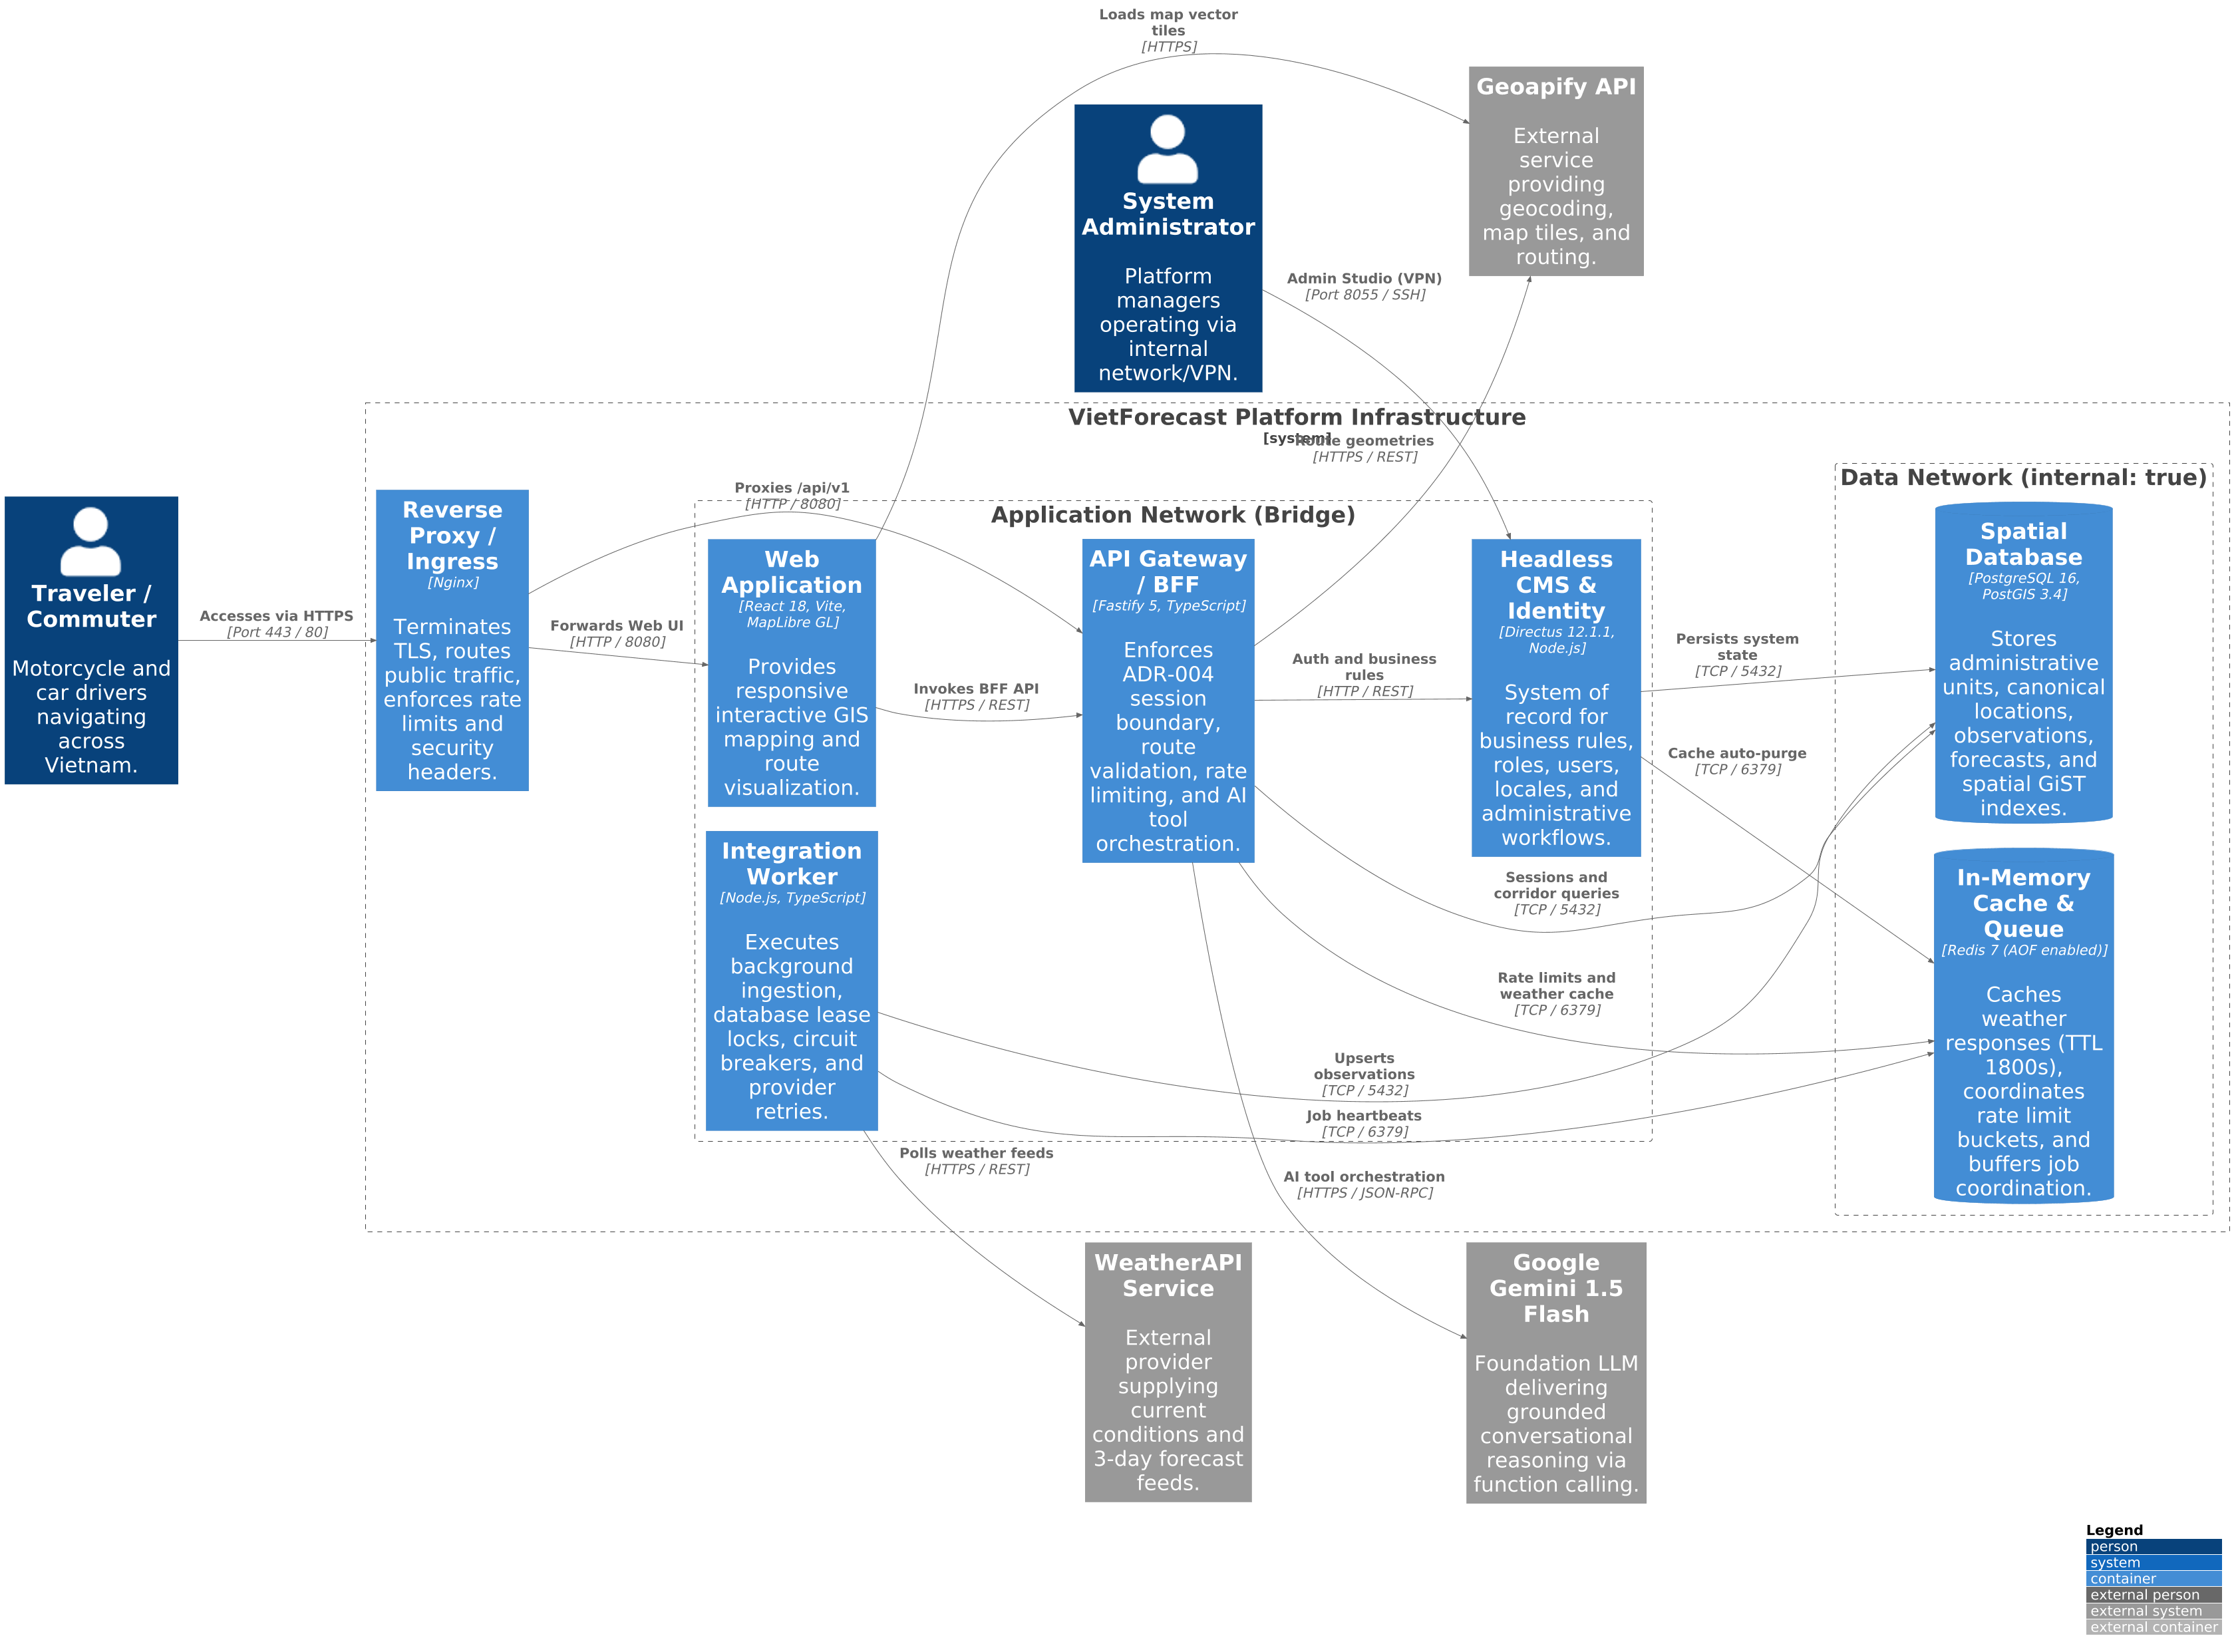
\includegraphics[width=0.95\textwidth, height=0.72\textheight, keepaspectratio]{figures/c4_container.png}
\caption[Biểu đồ C4 Container (Level 2) của VietForecast]{Biểu đồ C4 Container (Level 2) thể hiện cấu trúc microservices và phân vùng mạng của hệ thống VietForecast.}
\label{fig:c4_container_vi}
\end{figure}

Trách nhiệm kỹ thuật của từng container trong hệ thống được phân định rõ ràng theo nguyên tắc phân tách mối quan tâm (Separation of Concerns):
\begin{itemize}
    \item[-] Cổng đảo ngược và kết thúc mã hóa (\textit{Nginx Reverse Proxy}): Đóng vai trò là điểm tiếp nhận lưu lượng duy nhất từ Internet công cộng qua các cổng tiêu chuẩn 80 và 443. Thành phần này chịu trách nhiệm kết thúc phiên TLS/HTTPS, thiết lập các tiêu đề an ninh nghiêm ngặt (Content Security Policy, Strict-Transport-Security, X-Frame-Options), điều phối lưu lượng đến ứng dụng giao diện hoặc cổng giao tiếp API, và thực thi giới hạn lưu lượng truy cập ở cấp độ mạng để bảo vệ hạ tầng phía sau.
    \item[-] Ứng dụng giao diện web người dùng (\textit{Web Application}): Được phát triển dưới dạng ứng dụng trang đơn (Single Page Application) sử dụng React 18, trình đóng gói Vite và thư viện MapLibre GL 4. Ứng dụng cung cấp trải nghiệm tương tác bản đồ không gian mượt mà với tần số quét 60 khung hình trên giây nhờ tăng tốc phần cứng WebGL, trực quan hóa các lớp phủ khí tượng raster và hiển thị đa tuyến lộ trình ba chiều. Ứng dụng hoàn toàn không lưu trữ bất kỳ khóa bí mật API nào của nhà cung cấp bên thứ ba và không tiếp cận trực tiếp cơ sở dữ liệu.
    \item[-] Cổng giao tiếp dịch vụ và Điều phối nghiệp vụ (\textit{Fastify API / BFF}): Xây dựng trên nền tảng Fastify 5 và ngôn ngữ TypeScript, đóng vai trò là tầng trung gian Backend-For-Frontend (BFF). Thành phần này tiếp nhận các yêu cầu từ giao diện web, thực thi xác thực phiên làm việc, phân quyền người dùng, kiểm tra hạn mức sử dụng (rate limiting), điều phối thuật toán đánh giá rủi ro tuyến đường và làm cầu nối bảo mật gọi hàm có kiểm chứng (function calling) tới mô hình ngôn ngữ lớn Google Gemini 1.5 Flash.
    \item[-] Hệ quản trị nội dung và Danh tính người dùng (\textit{Directus 12.1.1}): Đóng vai trò là nguồn dữ liệu chân lý nghiệp vụ (System of Record) cho hệ thống tài khoản, phân quyền dựa trên vai trò (RBAC), danh mục đơn vị hành chính 63 tỉnh thành, các ngưỡng quy tắc rủi ro và nội dung bản địa hóa đa ngôn ngữ. Phiên bản Directus được ấn định chính xác ở bản phát hành 12.1.1 nhằm duy trì tính ổn định tuyệt đối về mặt lược đồ dữ liệu và giao diện quản trị Directus Admin Studio.
    \item[-] Tiến trình xử lý nền tích hợp (\textit{Integration Worker}): Là dịch vụ Node.js chạy độc lập, chịu trách nhiệm thực thi các tác vụ định kỳ có độ trễ cao và phụ thuộc mạng ngoài, bao gồm: thu thập dữ liệu thời tiết bề mặt và dự báo từ WeatherAPI, chuẩn hóa dữ liệu theo quy chuẩn WMO, tính toán giá trị băm kiểm tra tính toàn vẹn SHA-256, và cập nhật trạng thái làm mới vào cơ sở dữ liệu không gian.
    \item[-] Cơ sở dữ liệu không gian quan hệ (\textit{PostgreSQL 16 + PostGIS 3.4}): Là kho lưu trữ dữ liệu bền vững duy nhất của hệ thống, hỗ trợ các kiểu dữ liệu hình học OGC và thuật toán tính toán cung trắc địa elipxoit. Chỉ mục không gian GiST (Generalized Search Tree) được thiết lập trên toàn bộ các cột tọa độ và ranh giới để bảo đảm tốc độ truy vấn hành lang đệm đạt thời gian đáp ứng dưới 50 mili-giây.
    \item[-] Bộ đệm trong bộ nhớ và Điều phối luồng (\textit{Redis 7}): Vận hành với cơ chế ghi nhật ký thay đổi liên tục AOF (Append-Only File), cung cấp bộ nhớ đệm truy xuất tốc độ cực cao cho dữ liệu thời tiết hiện tại (thời gian sống TTL 1.800 giây), điều phối thuật toán Token Bucket kiểm soát tần suất gọi API, và lưu trữ trạng thái đồng bộ giữa các cụm tiến trình.
\end{itemize}

\subsection{Chính sách Phân vùng Mạng và An ninh Mạng Nội bộ (Docker Network Segmentation)}
Để triệt tiêu nguy cơ tấn công lan truyền khi một thành phần bị xâm nhập, hạ tầng vùng chứa Docker của VietForecast thiết lập chính sách phân vùng mạng nghiêm ngặt với hai phân đoạn mạng độc lập:
\begin{itemize}
    \item[-] Phân đoạn mạng ứng dụng nội bộ (\texttt{application} network): Là mạng cầu nối (bridge network) phục vụ việc truyền thông nghiệp vụ giữa Nginx, Web frontend, Fastify API, Directus và Integration Worker. Các dịch vụ trong phân vùng này có thể gửi và nhận các yêu cầu HTTP/REST nội bộ thông qua tên miền dịch vụ được Docker DNS giải quyết cục bộ.
    \item[-] Phân đoạn mạng dữ liệu cô lập tuyệt đối (\texttt{data} network với chỉ thị \texttt{internal: true}): Đây là phân vùng mạng an ninh cấp cao nhất của hệ thống. Chỉ thị \texttt{internal: true} ngăn chặn hoàn toàn việc phân bổ cổng ra ngoài bảng định tuyến Internet của máy chủ chủ (host). Cổng 5432 của PostgreSQL và cổng 6379 của Redis chỉ lắng nghe trên mạng nội bộ này, hoàn toàn vô hình trước môi trường bên ngoài. Bất kỳ nỗ lực quét cổng hay tấn công dò quét mật khẩu từ Internet vào tầng cơ sở dữ liệu đều bị triệt tiêu từ cấp độ định tuyến mạng vùng chứa.
\end{itemize}

Bên cạnh đó, giao diện quản trị Directus Admin Studio (lắng nghe tại cổng 8055) được cấu hình liên kết vòng lặp cục bộ (loopback binding \texttt{127.0.0.1:8055}) theo quy chuẩn an ninh ADR-002 và OPS-010. Người quản trị hệ thống bắt buộc phải thiết lập đường hầm bảo mật SSH (SSH Tunnel) hoặc kết nối qua mạng riêng ảo nội bộ (VPN) mới có thể truy cập trang quản trị, ngăn chặn nguy cơ bị tấn công brute-force hoặc khai thác lỗ hổng zero-day trên giao diện quản trị công khai.

\section{Thiết kế Ranh giới Phiên Bảo mật và An ninh Danh tính (ADR-004)}
\label{sec:auth_session_boundary}

\subsection{Phân tích Nguy cơ Đánh cắp Token và Kiến trúc Ranh giới Phiên BFF}
\label{subsec:token_threat_analysis_vi}
Trong các kiến trúc Single Page Application (SPA) truyền thống, mã xác thực JSON Web Token (Access Token và Refresh Token) \cite{rfc7519} thường được lưu trữ trực tiếp trong bộ nhớ trình duyệt (\texttt{localStorage} hoặc \texttt{sessionStorage}). Kiến trúc này bộc lộ lỗ hổng an ninh chí mạng: bất kỳ cuộc tấn công tiêm mã độc kịch bản chéo trang (Cross-Site Scripting -- XSS) nào bắt nguồn từ các gói phụ thuộc bên thứ ba đều cho phép mã độc chiếm đoạt trực tiếp JWT, dẫn tới việc mạo danh tài khoản mà máy chủ không thể phát hiện hay ngăn chặn. Ngoài ra, việc để máy khách giao tiếp trực tiếp với dịch vụ định danh Directus làm lộ cấu trúc lược đồ dữ liệu nội bộ và tạo sự gắn kết lỏng lẻo về mặt bảo mật.

Để khắc phục triệt để, nền tảng VietForecast thiết lập mô hình Backend-For-Frontend (BFF) thông qua Fastify API theo quyết định kiến trúc ADR-004. Fastify đóng vai trò là ranh giới phiên bảo mật duy nhất: toàn bộ việc giao tiếp với Directus diễn ra trong mạng nội bộ, trong khi trình duyệt tuyệt đối không bao giờ được tiếp cận hay lưu trữ mã JWT thô.

\subsection{Cơ chế Phong bì Mã hóa AES-256-GCM và Khóa Phiên Đục mờ}
\label{subsec:crypto_envelope_vi}
Hệ thống hiện thực hóa nguyên lý phân lập token nghiêm ngặt (\textit{Token Isolation}) và phòng thủ chiều sâu (\textit{Defense-in-Depth}) thông qua mô hình phong bì mật mã ba lớp:
\begin{itemize}
    \item[-] Khóa phiên ngẫu nhiên đục mờ (\textit{Opaque Session Handle}): Máy chủ Fastify phát sinh một chuỗi ngẫu nhiên giả mật mã dài 32 byte ($256\text{ bits}$) sử dụng bộ sinh số ngẫu nhiên CSPRNG (\texttt{createOpaque}\allowbreak\texttt{Token(32)}). Khóa phiên này được gửi về máy khách qua cookie \texttt{\_\_Host-\allowbreak vnwa\_\allowbreak session} với bốn cờ an ninh tối cao: \texttt{HttpOnly} (ngăn chặn JavaScript đọc qua \texttt{document.}\allowbreak\texttt{cookie}), \texttt{Secure} (bắt buộc truyền trên TLS/HTTPS), \texttt{SameSite=Strict} (vô hiệu hóa CSRF), và tiền tố \texttt{\_\_Host-} (khóa cookie vào đúng nguồn gốc tên miền).
    \item[-] Cơ chế băm khóa phiên một chiều (\textit{Token Hashing Pattern}): Nhằm bảo vệ trạng thái phiên ngay cả khi cơ sở dữ liệu bị trích xuất trái phép, máy chủ không lưu trực tiếp khóa đục mờ ở dạng rõ mà băm qua SHA-256 trước khi lưu vào bảng \texttt{app\_security.}\allowbreak\texttt{sessions}:
    \begin{equation}
    \label{eq:session_hash_vi}
    H_{\text{session}} = \text{SHA-256}(\text{handle})
    \end{equation}
    Bản băm $H_{\text{session}}$ dài 64 ký tự thập lục phân đóng vai trò là khóa chính (\texttt{session\_}\allowbreak\texttt{id\_}\allowbreak\texttt{hash}). Kẻ tấn công nếu chiếm được cơ sở dữ liệu cũng không thể giải mã ngược để tái tạo cookie phiên hợp lệ.
    \item[-] Phong bì mã hóa xác thực đối xứng AES-256-GCM (\textit{Authenticated Encryption Envelope}): Cặp mã Directus Access Token và Refresh Token được mã hóa phía máy chủ bằng thuật toán AES-256-GCM với khóa bí mật 256-bit ($K_{\text{enc}} \in \{0, 1\}^{256}$) do Fastify quản lý:
    \begin{equation}
    \label{eq:aes_gcm_vi}
    \mathcal{C} = \text{AES-GCM-Enc}_{K_{\text{enc}}}(P, \text{IV}), \quad \text{Tag} = \text{GCM-Mac}_{K_{\text{enc}}}(\mathcal{C}, \text{IV})
    \end{equation}
    Mỗi chu kỳ tạo hoặc xoay vòng khóa đều sinh một vectơ khởi tạo $\text{IV} \in \{0, 1\}^{96}$ (12 byte) ngẫu nhiên duy nhất và thẻ xác thực $\text{Tag} \in \{0, 1\}^{128}$ (16 byte). Cấu trúc phong bì lưu trữ tuần tự:
    \begin{equation}
    \label{eq:envelope_format_vi}
    \text{Envelope} = \texttt{v1} \,\|\, \text{base64url}(\text{IV}) \,\|\, \text{base64url}(\text{Tag}) \,\|\, \text{base64url}(\mathcal{C})
    \end{equation}
    Bản mã hóa và thẻ xác thực được lưu trữ bền vững trong bảng \texttt{app\_security.}\allowbreak\texttt{sessions}, với quyền truy cập chỉ phân bổ độc quyền cho tài khoản dịch vụ Fastify (\texttt{API\_}\allowbreak\texttt{DB\_}\allowbreak\texttt{USER}).
\end{itemize}

\subsection{Vòng đời Phiên Toàn diện: Cấp phát, Xoay vòng Trượt và Thu hồi Đồng bộ}
\label{subsec:auth_lifecycle_vi}
Vòng đời phiên bảo mật của người dùng được điều phối theo ba giai đoạn tuần tự và khép kín: xác thực cấp phát ban đầu, xoay vòng phiên trượt trơn tru trong quá trình tương tác, và thu hồi đồng bộ tức thời khi kết thúc phiên hoặc phát hiện bất thường an ninh.

\subsubsection{Giai đoạn 1: Xác thực danh tính và cấp phát khóa phiên đục mờ}
Hình~\ref{fig:seq_auth_lifecycle_p1_vi} biểu diễn chi tiết biểu đồ tuần tự của quy trình xác thực đăng nhập người dùng, cơ chế phân xử vai trò RBAC, bảo vệ chống cạn kiệt phiên và cấp phát cookie bảo mật \texttt{\_\_Host-\allowbreak vnwa\_\allowbreak session}.

\begin{figure}[H]
\centering
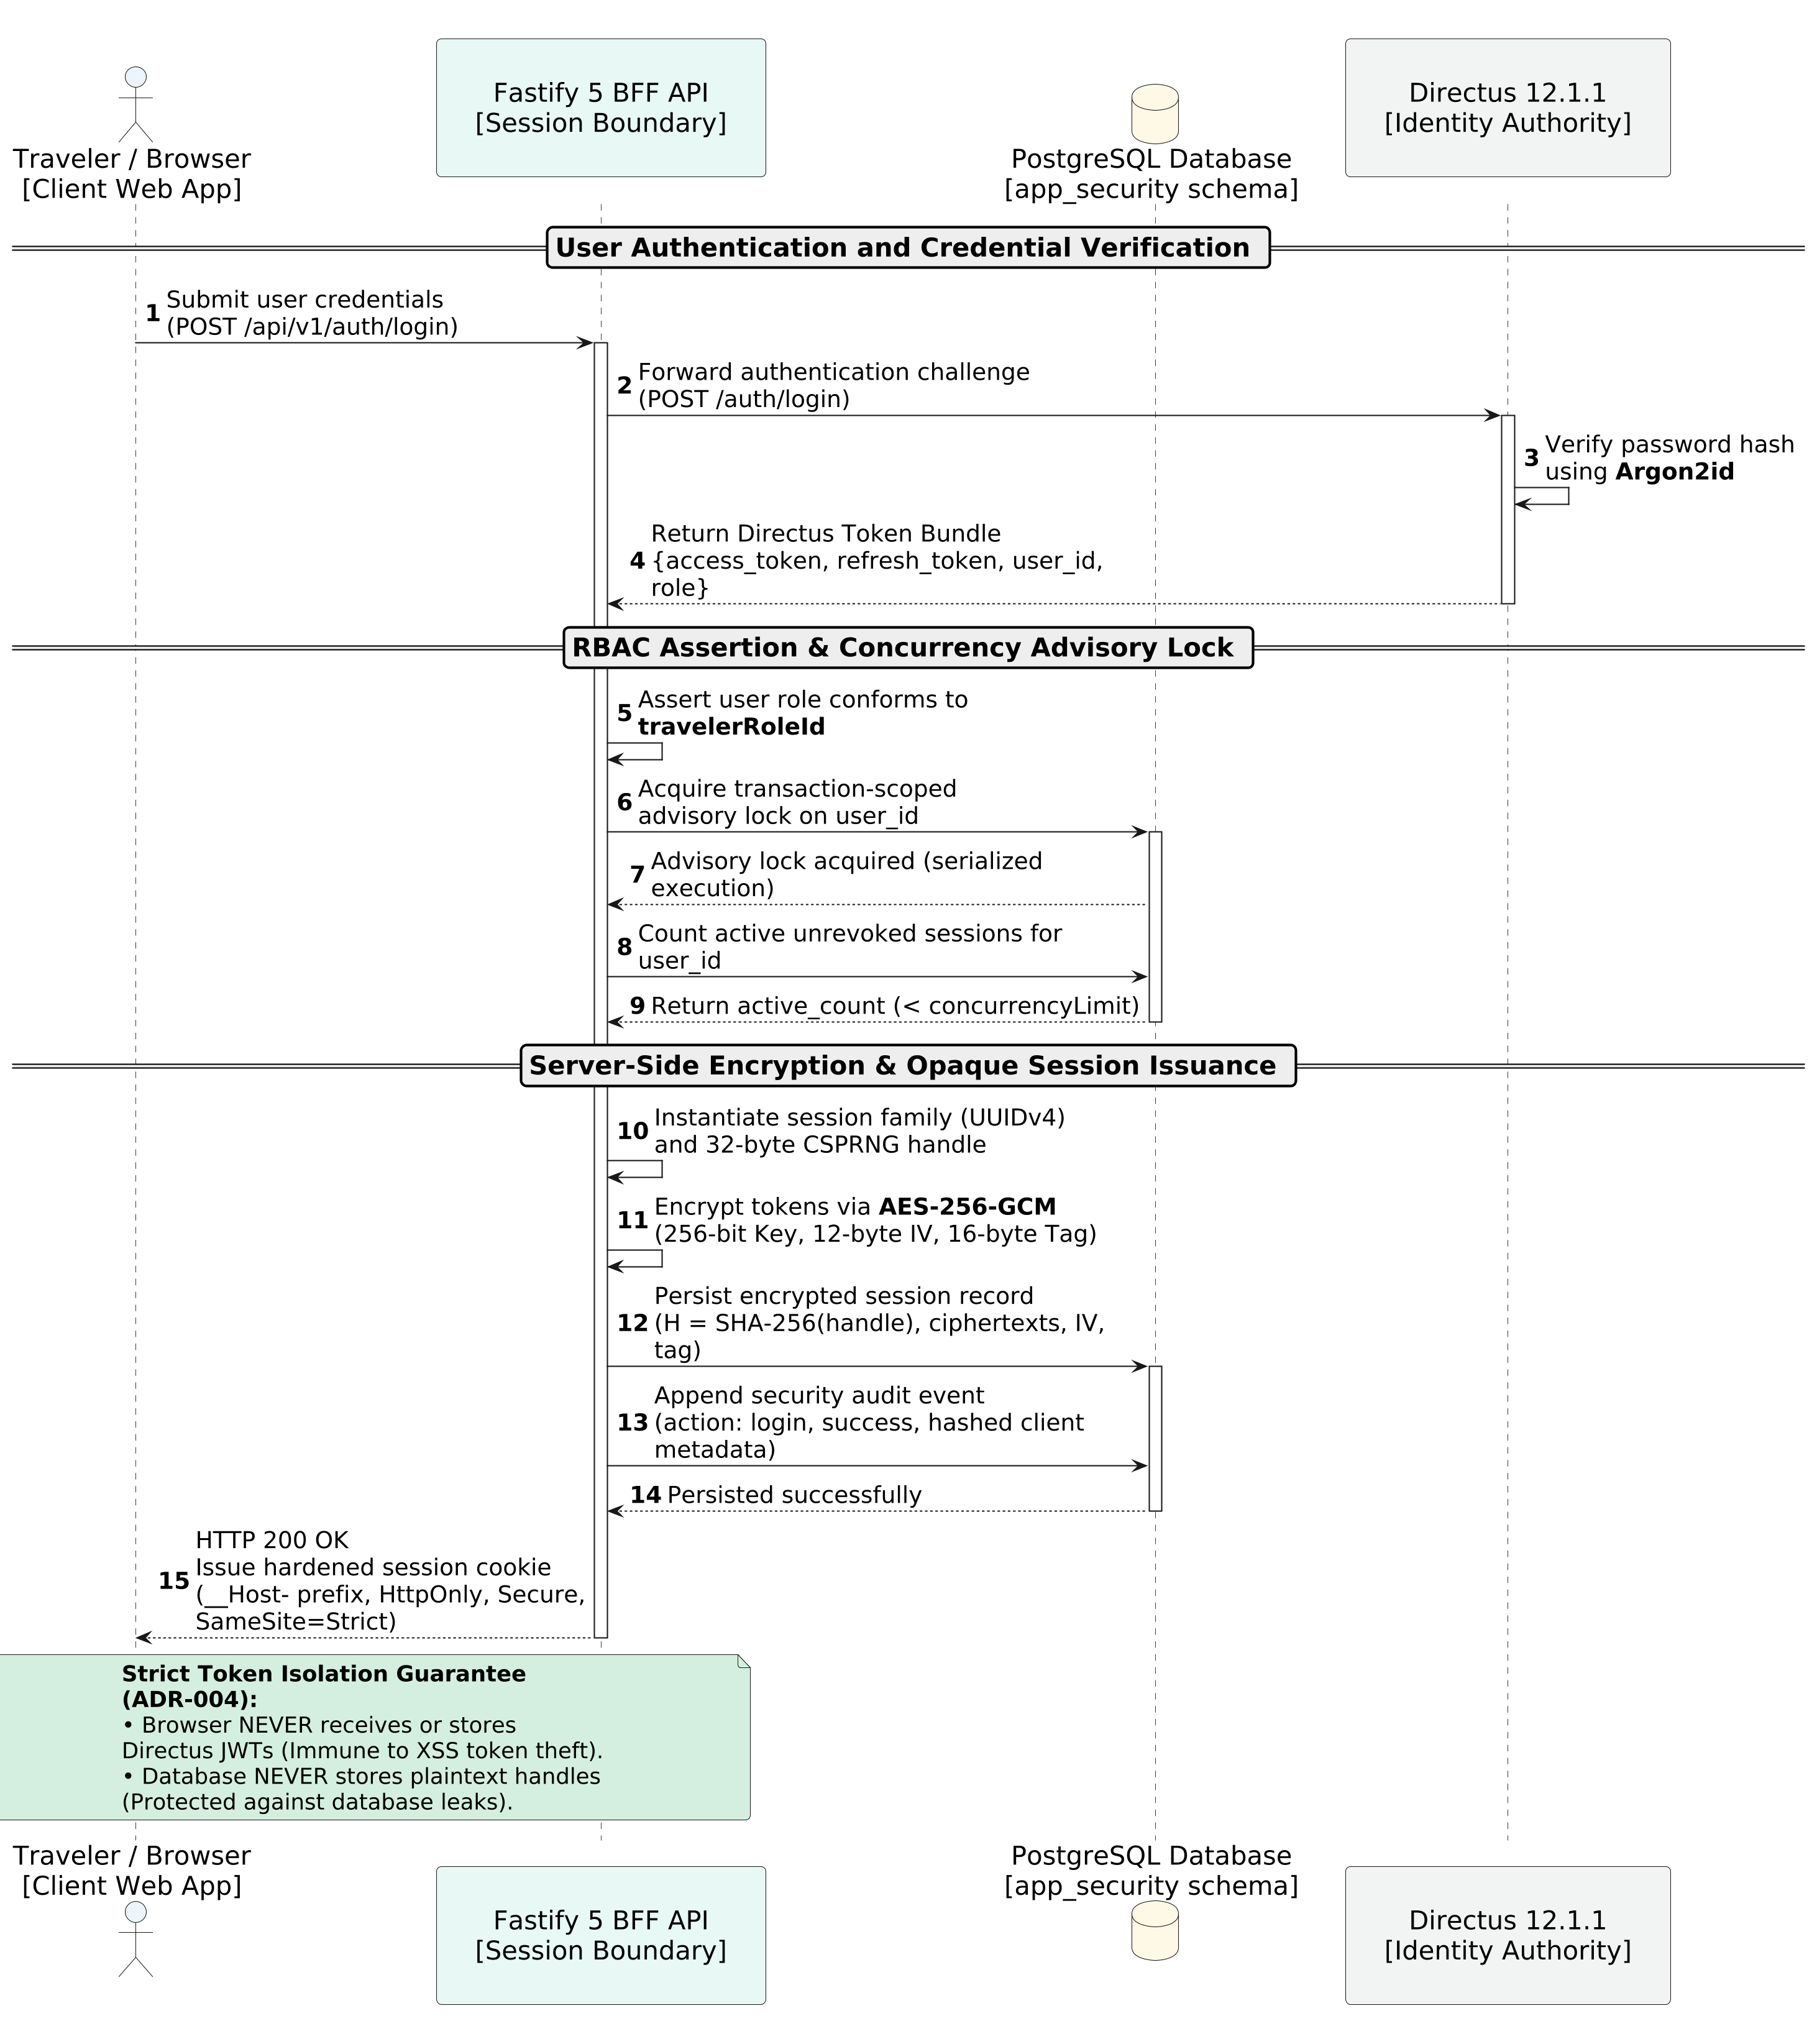
\includegraphics[width=0.92\textwidth, keepaspectratio]{figures/seq_auth_login.png}
\caption[Biểu đồ tuần tự vòng đời phiên (ADR-004) - Giai đoạn 1: Cấp phát khóa phiên]{Biểu đồ tuần tự vòng đời phiên (ADR-004) -- Giai đoạn 1: Xác thực đăng nhập người dùng, cơ chế phân xử vai trò RBAC, kiểm soát phiên đồng thời và cấp phát khóa phiên đục mờ.}
\label{fig:seq_auth_lifecycle_p1_vi}
\end{figure}

Flow hoạt động của Giai đoạn 1 diễn ra qua các bước tuần tự chuẩn hóa:
\begin{itemize}
    \item[-] \textit{Bước 1 (Gửi chứng thực đăng nhập)}: Người dùng nhập thông tin chứng thực (email và mật khẩu) trên ứng dụng giao diện web. Trình duyệt gửi yêu cầu \texttt{POST /api/v1/auth/login} tới cổng Fastify API. Fastify thực thi kiểm tra giới hạn tần suất gọi (Leaky Bucket, 5 req/phút) để ngăn chặn tấn công dò quét mật khẩu.
    \item[-] \textit{Bước 2 (Ủy nhiệm xác thực danh tính)}: Fastify chuyển tiếp thông tin tới Directus Identity Authority qua mạng nội bộ \texttt{application}. Directus kiểm tra mật khẩu đối chiếu với bản băm an toàn theo thuật toán Argon2id. Khi thông tin hợp lệ, Directus phát hành gói mã token gồm Access Token ngắn hạn, Refresh Token dài hạn, mã định danh người dùng và vai trò phân quyền.
    \item[-] \textit{Bước 3 (Thẩm định RBAC và khóa tư vấn phiên đồng thời)}: Fastify kiểm tra vai trò người dùng thuộc đúng nhóm \texttt{travelerRoleId}. Để ngăn chặn tấn công chiếm dụng tài nguyên phiên hoặc vượt quá số lượng thiết bị cho phép, hệ thống tuần tự hóa nguyên tử việc kiểm tra số lượng phiên hoạt động của người dùng $u$ thông qua khóa tư vấn cấp giao dịch (transaction-scoped advisory lock) liên kết với giá trị băm $h_u = \text{Hash}_{64}(u)$:
    \begin{equation}
    \label{eq:concurrency_bound_vi}
    N_{\text{active}}(u) = \Big| \big\{ s \in \mathcal{S} \;\big|\; s.\text{user\_id} = u \;\wedge\; s.\text{revoked\_at} = \emptyset \big\} \Big| < C_{\text{limit}}
    \end{equation}
    Nếu số lượng phiên chạm ngưỡng quy định $C_{\text{limit}}$, hệ thống tự động vô hiệu hóa phiên cũ nhất để giải phóng tài nguyên.
    \item[-] \textit{Bước 4 (Mã hóa phong bì AES-256-GCM và sinh khóa đục mờ)}: Fastify sinh định danh họ phiên mới (UUIDv4) cùng khóa phiên đục mờ ngẫu nhiên dài 32 byte ($h$) từ bộ sinh số ngẫu nhiên CSPRNG. Cặp mã JWT được đóng gói và mã hóa đối xứng phía máy chủ bằng thuật toán AES-256-GCM với vectơ khởi tạo ngẫu nhiên 12 byte ($\text{IV} \in \{0, 1\}^{96}$) và thẻ xác thực 16 byte ($\text{Tag} \in \{0, 1\}^{128}$) theo Khóa mã hóa máy chủ $K_{\text{enc}}$.
    \item[-] \textit{Bước 5 (Lưu trữ bản băm một chiều và ghi nhật ký kiểm toán)}: Fastify tính bản băm một chiều $H_{\text{session}} = \text{SHA-256}(h)$ và ghi bản ghi phiên vào bảng \texttt{app\_security.sessions}. Đồng thời, một bản ghi kiểm toán bất biến được ghi nhận vào bảng \texttt{app\_}\allowbreak\texttt{security.}\allowbreak\texttt{audit\_}\allowbreak\texttt{events} với hành động đăng nhập thành công kèm siêu dữ liệu máy khách đã băm bảo vệ quyền riêng tư.
    \item[-] \textit{Bước 6 (Phát hành cookie bảo mật)}: Fastify trả về phản hồi thành công (HTTP 200 OK) và thiết lập cookie phiên bảo mật \texttt{\_\_Host-vnwa\_session} trên trình duyệt với cờ \texttt{HttpOnly} (ngăn chặn JavaScript đọc cookie), cờ \texttt{Secure} (bắt buộc truyền tải trên kênh TLS), cờ \texttt{SameSite=Strict} (triệt tiêu tấn công CSRF) và tiền tố \texttt{\_\_Host-} (ràng buộc tuyệt đối nguồn gốc tên miền).
\end{itemize}

\subsubsection{Giai đoạn 2: Xử lý yêu cầu ủy quyền và xoay vòng phiên trượt trơn tru}
Hình~\ref{fig:seq_auth_lifecycle_p2_vi} minh họa chi tiết biểu đồ tuần tự của quy trình tiếp nhận yêu cầu ủy quyền nghiệp vụ và cơ chế xoay vòng phiên trượt ngầm (Silent Sliding Rotation).

\begin{figure}[H]
\ContinuedFloat
\centering
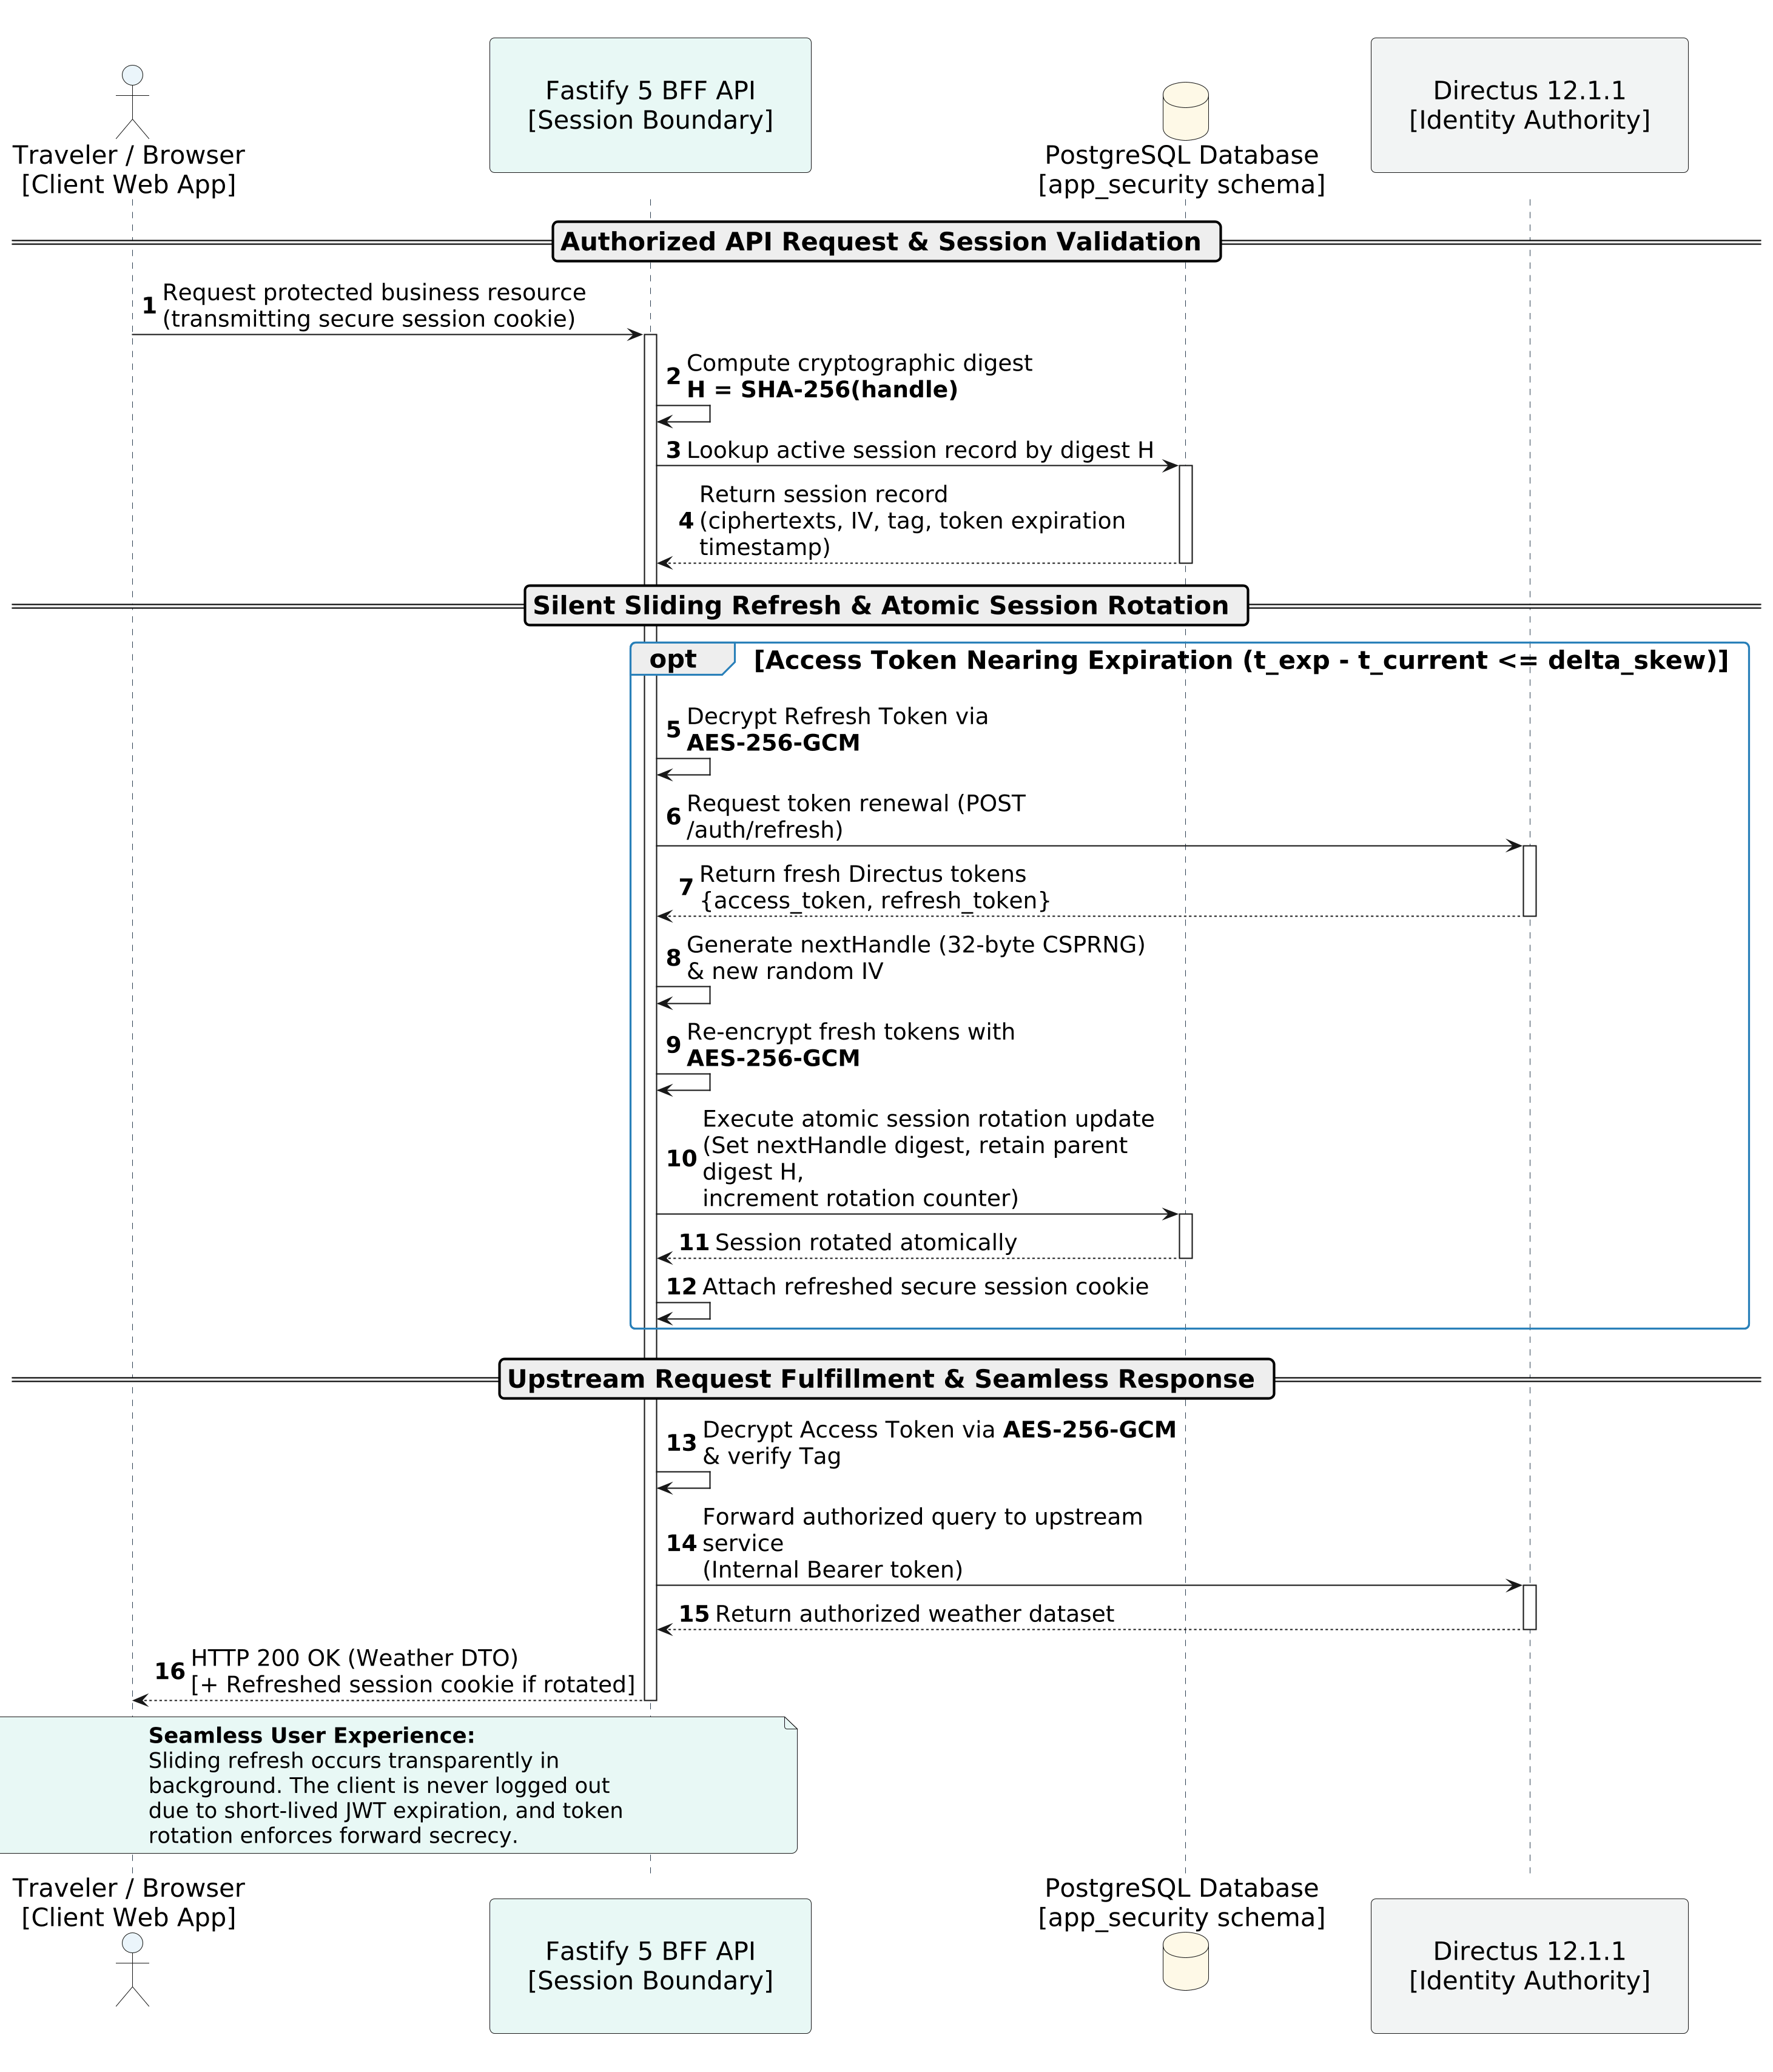
\includegraphics[width=0.92\textwidth, keepaspectratio]{figures/seq_sliding_rotation.png}
\caption[Biểu đồ tuần tự vòng đời phiên (ADR-004) - Giai đoạn 2: Xoay vòng trượt ngầm]{Biểu đồ tuần tự vòng đời phiên (ADR-004) (tiếp theo) -- Giai đoạn 2: Xử lý yêu cầu ủy quyền nghiệp vụ và cơ chế xoay vòng phiên trượt trơn tru (Silent Sliding Rotation).}
\label{fig:seq_auth_lifecycle_p2_vi}
\end{figure}

Flow hoạt động của Giai đoạn 2 được thiết kế như sau:
\begin{itemize}
    \item[-] \textit{Bước 1 (Đón bắt cookie và đối chiếu bản băm)}: Khi máy khách gửi yêu cầu nghiệp vụ kèm theo cookie \texttt{\_\_Host-\allowbreak vnwa\_\allowbreak session}, tầng chặn bắt an ninh của Fastify trích xuất chuỗi định danh phiên $h$, tính bản băm $H = \text{SHA-256}(h)$, và đối chiếu với tập trạng thái phiên trong cơ sở dữ liệu (hoặc bộ đệm Redis). Nếu không tồn tại bản ghi hợp lệ hoặc phiên đã bị đánh dấu thu hồi, yêu cầu lập tức bị từ chối với mã lỗi HTTP 401 Unauthorized.
    \item[-] \textit{Bước 2 (Đánh giá cửa sổ dung sai làm mới trượt)}: Sau khi xác thực phiên hợp lệ, Fastify kiểm tra thời hạn sống còn lại của Access Token trong phong bì mã hóa. Nếu khoảng cách từ thời điểm hiện tại $t_{\text{current}}$ đến mốc hết hạn $t_{\text{exp}}$ nhỏ hơn hoặc bằng ngưỡng dung sai làm mới $\Delta t_{\text{skew}}$:
    \begin{equation}
    \label{eq:sliding_skew_vi}
    t_{\text{exp}} - t_{\text{current}} \le \Delta t_{\text{skew}}
    \end{equation}
    hệ thống tự động kích hoạt luồng làm mới phiên trượt ngầm hoàn toàn trong suốt với người dùng.
    \item[-] \textit{Bước 3 (Đổi token và chuyển dịch trạng thái nguyên tử)}: Fastify sử dụng khóa $K_{\text{enc}}$ giải mã Refresh Token bằng thuật toán AES-256-GCM và gọi nội bộ sang Directus để đổi lấy cặp token mới. Ngay sau khi nhận cặp token mới, Fastify sinh một khóa phiên đục mờ kế tiếp $h_{k+1}$ dài 32 byte và vectơ khởi tạo $\text{IV}_{k+1}$ mới để tái mã hóa gói dữ liệu. Quá trình xoay vòng chuyển dịch trạng thái nguyên tử qua toán tử $\mathcal{T}_{\text{rotate}}$:
    \begin{equation}
    \label{eq:rotate_session_vi}
    \begin{aligned}
    \mathcal{T}_{\text{rotate}}(S_k) \xrightarrow{\text{nguyên tử}} S_{k+1} = \big\langle & \text{SHA-256}(h_{k+1}),\; \mathcal{C}_{k+1}, \\
    & \text{IV}_{k+1},\; \text{Tag}_{k+1},\; t_{\text{exp}, k+1},\; c_k + 1 \big\rangle
    \end{aligned}
    \end{equation}
    đồng thời duy trì liên kết phả hệ khóa cha để phát hiện tấn công tái sử dụng:
    \begin{equation}
    \label{eq:rotate_lineage_vi}
    S_{k+1}.\text{ancestor\_hash} = H_k
    \end{equation}
    \item[-] \textit{Bước 4 (Thời gian ân hạn và hoàn tất yêu cầu nghiệp vụ)}: Khóa phiên cũ $h_k$ được duy trì trong một khoảng thời gian ân hạn ngắn ($\text{TTL}_{\text{grace}} = 60\text{ s}$) trong Redis nhằm xử lý các yêu cầu mạng đồng thời đang bay dở dang mà không gây lỗi phiên giả mạo. Fastify giải mã Access Token, gắn vào tiêu đề ủy quyền nội bộ để truy vấn tập dữ liệu thời tiết, và trả kết quả về cho máy khách kèm theo chỉ thị cập nhật cookie phiên mang khóa thế hệ mới $h_{k+1}$.
\end{itemize}

\subsubsection{Giai đoạn 3: Thu hồi phiên đồng bộ và tiêu hủy phả hệ phiên}
Hình~\ref{fig:seq_auth_lifecycle_p3_vi} minh họa biểu đồ tuần tự của cơ chế thu hồi phiên đồng bộ qua Trigger cơ sở dữ liệu và tiêu hủy họ phiên khi phát hiện tái sử dụng token.

\begin{figure}[H]
\ContinuedFloat
\centering
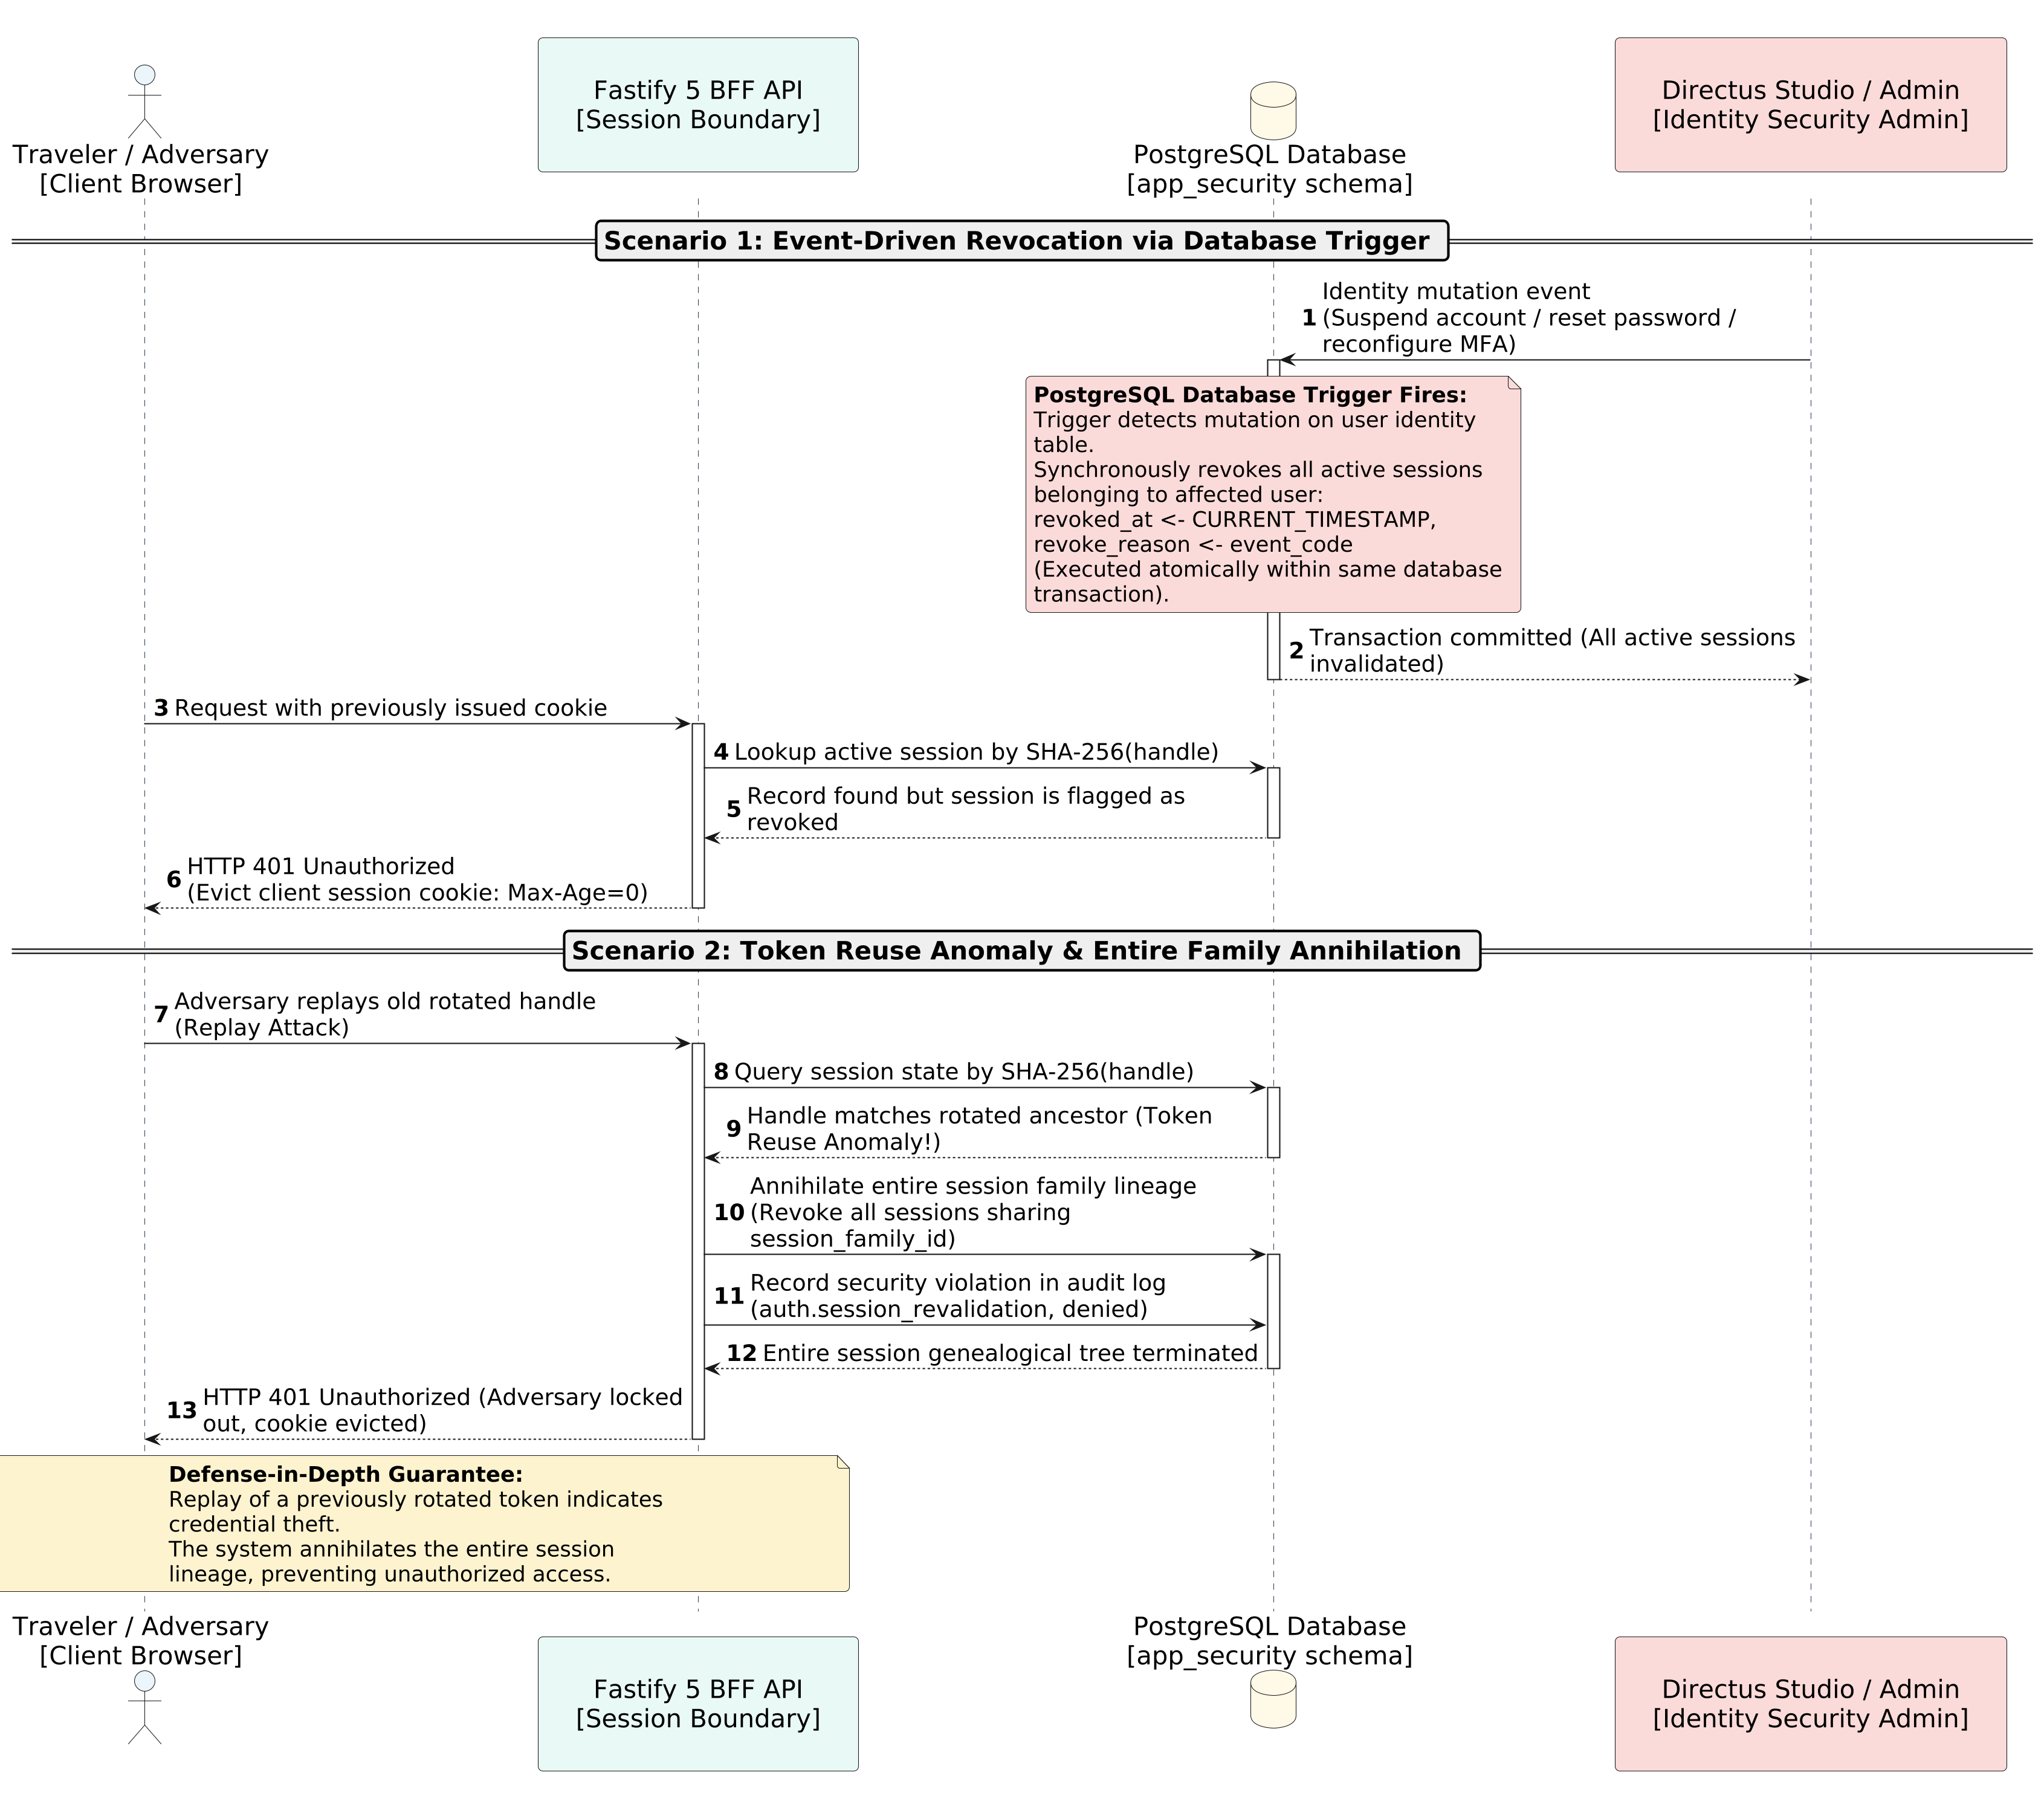
\includegraphics[width=0.92\textwidth, keepaspectratio]{figures/seq_session_revocation.png}
\caption[Biểu đồ tuần tự vòng đời phiên (ADR-004) - Giai đoạn 3: Thu hồi đồng bộ]{Biểu đồ tuần tự vòng đời phiên (ADR-004) (tiếp theo) -- Giai đoạn 3: Thu hồi họ phiên đồng bộ qua Trigger cơ sở dữ liệu và tiêu hủy toàn bộ dòng họ phiên khi phát hiện tái sử dụng token.}
\label{fig:seq_auth_lifecycle_p3_vi}
\end{figure}

Flow hoạt động của Giai đoạn 3 được điều phối qua ba kịch bản phòng thủ chuyên sâu:
\begin{itemize}
    \item[-] \textit{Kịch bản 1 (Thu hồi đồng bộ hướng sự kiện qua Trigger cơ sở dữ liệu)}: Khi người quản trị thực hiện vô hiệu hóa tài khoản trên Directus Studio, hoặc khi người dùng đổi mật khẩu hay cập nhật cấu hình xác thực hai yếu tố (MFA), một biến cố đột biến danh tính xảy ra. Trigger cơ sở dữ liệu tự động kích hoạt toán tử vô hiệu hóa $\Phi_{\text{trigger}}$ trong cùng một giao dịch ACID:
    \begin{equation}
    \label{eq:trigger_revoke_vi}
    \begin{aligned}
    \forall s \in \mathcal{S}, \; (s.\text{user\_id} = u \;\wedge\; s.\text{revoked\_at} = \emptyset) \implies \\
    \Phi_{\text{trigger}}(s) : \begin{cases}
    s.\text{revoked\_at} \leftarrow t_{\text{event}} \\
    s.\text{revoke\_reason} \leftarrow \text{code}_{\text{reason}}
    \end{cases}
    \end{aligned}
    \end{equation}
    trong đó $t_{\text{event}}$ là thời điểm giao dịch danh tính diễn ra, và $\text{code}_{\text{reason}}$ là mã nguyên nhân chuẩn hóa (\texttt{identity\_}\allowbreak\texttt{password\_}\allowbreak\texttt{changed}, \texttt{identity\_}\allowbreak\texttt{status\_}\allowbreak\texttt{changed}, \texttt{identity\_}\allowbreak\texttt{role\_}\allowbreak\texttt{changed}, \texttt{identity\_}\allowbreak\texttt{mfa\_}\allowbreak\texttt{changed}, hoặc \texttt{identity\_}\allowbreak\texttt{deleted}). Toàn bộ các phiên đang hoạt động của người dùng trên mọi thiết bị lập tức bị vô hiệu hóa đồng loạt.
    \item[-] \textit{Kịch bản 2 (Phát hiện tái sử dụng token và tiêu hủy toàn bộ họ phiên)}: Nếu kẻ tấn công đánh cắp được một cookie phiên cũ đã qua xoay vòng và cố gắng gửi yêu cầu sau khi thời gian ân hạn 60 giây đã kết thúc, Fastify phát hiện giá trị băm của cookie trùng khớp với trường lưu vết khóa cha $S.\text{ancestor\_hash}$ của một bản ghi đã tiến hóa. Fastify lập tức kích hoạt toán tử tiêu hủy toàn bộ dòng họ phiên $\Psi_{\text{annihilate}}$:
    \begin{equation}
    \label{eq:family_revoke_vi}
    \begin{aligned}
    \forall s \in \mathcal{S}, \; (s.\text{family\_id} = F_{\text{target}}) \implies \\
    \Psi_{\text{annihilate}}(s) : \begin{cases}
    s.\text{revoked\_at} \leftarrow t_{\text{detection}} \\
    s.\text{revoke\_reason} \leftarrow \text{`token\_reuse\_detected'}
    \end{cases}
    \end{aligned}
    \end{equation}
    Đồng thời, toàn bộ khóa liên đới trong Redis bị xóa sạch và một cảnh báo an ninh nghiêm trọng được ghi vào nhật ký kiểm toán, trung hòa hoàn toàn nguy cơ kẻ tấn công lợi dụng phiên bị rò rỉ.
    \item[-] \textit{Kịch bản 3 (Đăng xuất tự nguyện và thanh trừng định kỳ)}: Khi người dùng bấm đăng xuất (\texttt{POST /auth/logout}), Fastify cập nhật trường \texttt{revoked\_at} trong cơ sở dữ liệu, xóa khóa đệm trong Redis và phát lệnh xóa cookie \texttt{\_\_Host-vnwa\_session} (thiết lập \texttt{Max-Age=0}). Thủ tục dọn dẹp định kỳ chạy ngầm thực hiện thanh trừng vĩnh viễn các bản ghi phiên đã thu hồi vượt quá thời gian lưu trữ bắt buộc.
\end{itemize}

\section{Thiết kế Tiến trình Xử lý Nền Worker và Cơ chế Ổn định Hệ thống (ADR-001)}
\label{sec:worker_resilience_adr001}

\subsection{Phân tách Miền Lỗi Giữa Tác vụ Nền và Giao diện Lập trình Ứng dụng}
Trong quá trình vận hành hệ thống thông tin khí tượng, tác vụ thu thập dữ liệu từ các dịch vụ API bên ngoài (như WeatherAPI) có xác suất gặp lỗi cao do nghẽn mạng quốc tế, quá tải máy chủ cung cấp hoặc cạn kiệt hạn ngạch truy vấn. Hơn nữa, việc thu thập dữ liệu cho toàn bộ 63 tỉnh thành Việt Nam với chu kỳ 15 đến 30 phút một lần tiêu tốn đáng kể thời gian I/O và chu kỳ xử lý chuẩn hóa dữ liệu.

Nếu tích hợp các tác vụ này vào trong cùng một tiến trình ứng dụng API phục vụ người dùng hoặc tận dụng luồng tự động hóa (Directus Flow) kéo dài, hiện tượng tranh chấp tài nguyên (Event Loop Blocking) sẽ xảy ra, làm giảm sút nghiêm trọng tốc độ phản hồi các yêu cầu tương tác giao diện và có thể dẫn đến sự cố sập đổ dây chuyền (Cascading Failure). Do đó, theo quyết định kiến trúc ADR-001, toàn bộ các tác vụ thu thập, chuẩn hóa, tính toán và bảo trì dữ liệu được phân tách hoàn toàn sang một tiến trình xử lý nền độc lập mang tên Integration Worker.

\subsection{Cơ chế Chiếm Khóa Phân tán trên Cơ sở Dữ liệu (Distributed Database Leasing)}
Để ngăn chặn tình trạng nhiều tiến trình worker cùng thực thi thu thập dữ liệu trùng lặp khi hệ thống được mở rộng ngang trên nhiều container hoặc nhiều máy chủ vật lý, hệ thống triển khai cơ chế chiếm khóa phân tán (Distributed Database Leasing) trên bảng \texttt{weather\_worker\_leases} của PostgreSQL.

Cơ chế này hoạt động dựa trên nguyên tắc chiếm quyền độc quyền có thời hạn (atomic acquisition with expiration):
\begin{itemize}
    \item[-] Khi bắt đầu một chu kỳ đồng bộ dữ liệu, worker cố gắng thực thi câu lệnh chèn hoặc cập nhật có điều kiện (\texttt{INSERT ... ON CONFLICT DO UPDATE}) trên bản ghi khóa tài nguyên. Thao tác chỉ thành công nếu chưa có worker nào nắm giữ khóa hoặc khóa hiện tại đã vượt quá thời gian hiệu lực (hết hạn).
    \item[-] Thời gian giữ khóa được quy định bởi tham số \texttt{WEATHER\_}\allowbreak\texttt{WORKER\_}\allowbreak\texttt{LEASE\_}\allowbreak\texttt{DURATION\_MS} ($120.000\text{ ms}$).
    \item[-] Trong suốt quá trình thực thi tác vụ tải dữ liệu và chuẩn hóa, worker định kỳ gửi tín hiệu nhịp tim (\texttt{heartbeat}) sau mỗi 30.000 mili-giây (\texttt{HEARTBEAT\_INTERVAL\_MS} ($30.000\text{ ms}$)) để gia hạn thời điểm hết hạn của khóa.
    \item[-] Trong trường hợp tiến trình worker bị sập nguồn đột ngột hoặc mất kết nối mạng, tín hiệu nhịp tim bị gián đoạn. Khi vượt quá ngưỡng 120 giây, khóa tự động bị coi là hết hạn mà không gây ra tình trạng bế tắc vĩnh viễn (deadlock). Tiến trình worker kế tiếp có thể tiếp quản tài nguyên và thực thi chu kỳ đồng bộ tiếp theo một cách an toàn và tự động.
\end{itemize}

\subsection{Cơ chế Ngắt mạch (Circuit Breaker) và Thử lại Thích ứng}
Để bảo vệ hạn mức truy vấn API thời tiết của hệ thống cũng như duy trì tính sẵn sàng khi dịch vụ ngoài gặp sự cố, tiến trình Integration Worker tích hợp mô hình ngắt mạch (Circuit Breaker Pattern) ba trạng thái:
\begin{itemize}
    \item[-] \textit{Trạng thái Đóng (CLOSED)}: Toàn bộ các yêu cầu gọi sang WeatherAPI được thực thi bình thường. Hệ thống giám sát tỷ lệ lỗi liên tiếp.
    \item[-] \textit{Trạng thái Mở (OPEN)}: Khi số lần gọi thất bại liên tiếp (do lỗi mã phản hồi HTTP 5xx, lỗi quá tải HTTP 429 hoặc vượt quá thời gian chờ \texttt{TIMEOUT\_MS} ($8.000\text{ ms}$)) chạm ngưỡng \texttt{CIRCUIT\_FAILURE\_}\allowbreak\texttt{THRESHOLD} ($3$ lần), bộ ngắt mạch lập tức chuyển sang trạng thái Mở. Trong trạng thái này, mọi yêu cầu thu thập dữ liệu mới bị đình chỉ ngay lập tức tại worker mà không gửi yêu cầu ra mạng bên ngoài, giúp bảo toàn tài nguyên và tránh gây áp lực thêm lên máy chủ nhà cung cấp.
    \item[-] \textit{Trạng thái Bán Mở (HALF-OPEN)}: Sau thời gian chờ \texttt{CIRCUIT\_RESET\_MS} ($60.000\text{ ms}$) (60 giây), bộ ngắt mạch tự động chuyển sang trạng thái Bán Mở và cho phép một yêu cầu thăm dò đơn lẻ được phát đi. Nếu yêu cầu này thành công, mạch quay về trạng thái Đóng; ngược lại nếu tiếp tục thất bại, mạch tái lập trạng thái Mở và khởi động lại chu kỳ đếm thời gian.
\end{itemize}

Đối với các lỗi mang tính nhất thời, worker kích hoạt thuật toán thử lại theo hàm số mũ kết hợp độ trễ ngẫu nhiên (Exponential Backoff with Jitter). Khoảng thời gian trì hoãn giữa các lần thử lại thứ $k$ được tính toán theo công thức:
\begin{equation}
\label{eq:backoff_jitter}
t_{\text{delay}}(k) = \min\left(t_{\max}, \; t_{\text{base}} \cdot 2^{k-1}\right) \cdot \left(1 + r_{\text{jitter}} \cdot \mathcal{U}(-1, 1)\right)
\end{equation}
với độ trễ cơ sở $t_{\text{base}} = 5.000\text{ ms}$, độ trễ trần $t_{\max} = 60.000\text{ ms}$, tỷ lệ độ trễ ngẫu nhiên $r_{\text{jitter}} = 0{,}2$ và $\mathcal{U}(-1, 1)$ là biến ngẫu nhiên phân bố đều trong khoảng $[-1, 1]$. Yếu tố ngẫu nhiên này đóng vai trò quyết định trong việc ngăn chặn hiện tượng nghẽn mạng tập trung (thundering herd problem) khi nhiều trạm thời tiết cùng đồng loạt thử kết nối lại tại một thời điểm.

\subsection{Kiểm soát Vòng đời Độ tươi mới Dữ liệu Khí tượng và Trạng thái An toàn}
Dữ liệu quan trắc sau khi thu thập thành công từ WeatherAPI được chuẩn hóa về hệ thống đơn vị đo lường khí tượng quốc tế (WMO-No. 8) và tính toán mã băm SHA-256 để chống trùng lặp dữ liệu trước khi ghi vào bảng \texttt{weather\_}\allowbreak\texttt{observations}. Đồng thời, worker cập nhật bản ghi trong bảng dự báo \texttt{weather\_forecasts} và phát tín hiệu làm mới bộ nhớ đệm Redis với thời gian sống TTL tương ứng.

Dữ liệu thời tiết lưu trữ trong hệ thống được kiểm soát nghiêm ngặt theo ba trạng thái độ tươi mới nhằm bảo đảm tính an toàn cho động cơ tính điểm rủi ro hành trình:
\begin{itemize}
    \item[-] \textit{Dữ liệu mới (Fresh)}: Độ trễ $\tau \le 60$ phút tính từ thời điểm đo thực tế tại trạm quan trắc. Dữ liệu này được coi là hoàn toàn hợp lệ và phản ánh chính xác tình trạng khí quyển hiện tại, được đưa trực tiếp vào thuật toán đánh giá an toàn lộ trình.
    \item[-] \textit{Dữ liệu cũ (Aging)}: Độ trễ nằm trong khoảng $60 < \tau \le 180$ phút. Hệ thống vẫn cho phép truy vấn phục vụ các tính toán định tuyến nhưng giao diện ứng dụng bắt buộc hiển thị nhãn cảnh báo thời điểm cập nhật cũ để người dùng chủ động lưu ý.
    \item[-] \textit{Dữ liệu hết hạn (Stale)}: Khi độ trễ $\tau > 180$ phút (hoặc trạm quan trắc mất kết nối quá 3 giờ). Theo nguyên tắc thiết kế an toàn tuyệt đối (Fail-Safe Principle), hệ thống kiên quyết từ chối sử dụng dữ liệu này để nội suy rủi ro và tự động ánh xạ mức độ nguy hiểm về trạng thái \texttt{Unknown} (mã màu xám \#9CA3AF), bảo đảm người tham gia giao thông luôn nhận thức rõ việc thiếu dữ liệu thực địa thay vì tin tưởng vào các dự báo an toàn giả tạo.
\end{itemize}

Hình~\ref{fig:seq_ingestion_vi} mô tả chi tiết toàn bộ chu trình vận hành nền của tiến trình Integration Worker, bao gồm cơ chế chiếm quyền khóa phân tán, xử lý ngắt mạch tự động khi có lỗi mạng, khâu kiểm tra toàn vẹn mã băm và cập nhật giao dịch ACID vào hệ thống lưu trữ.

\begin{figure}[H]
\centering
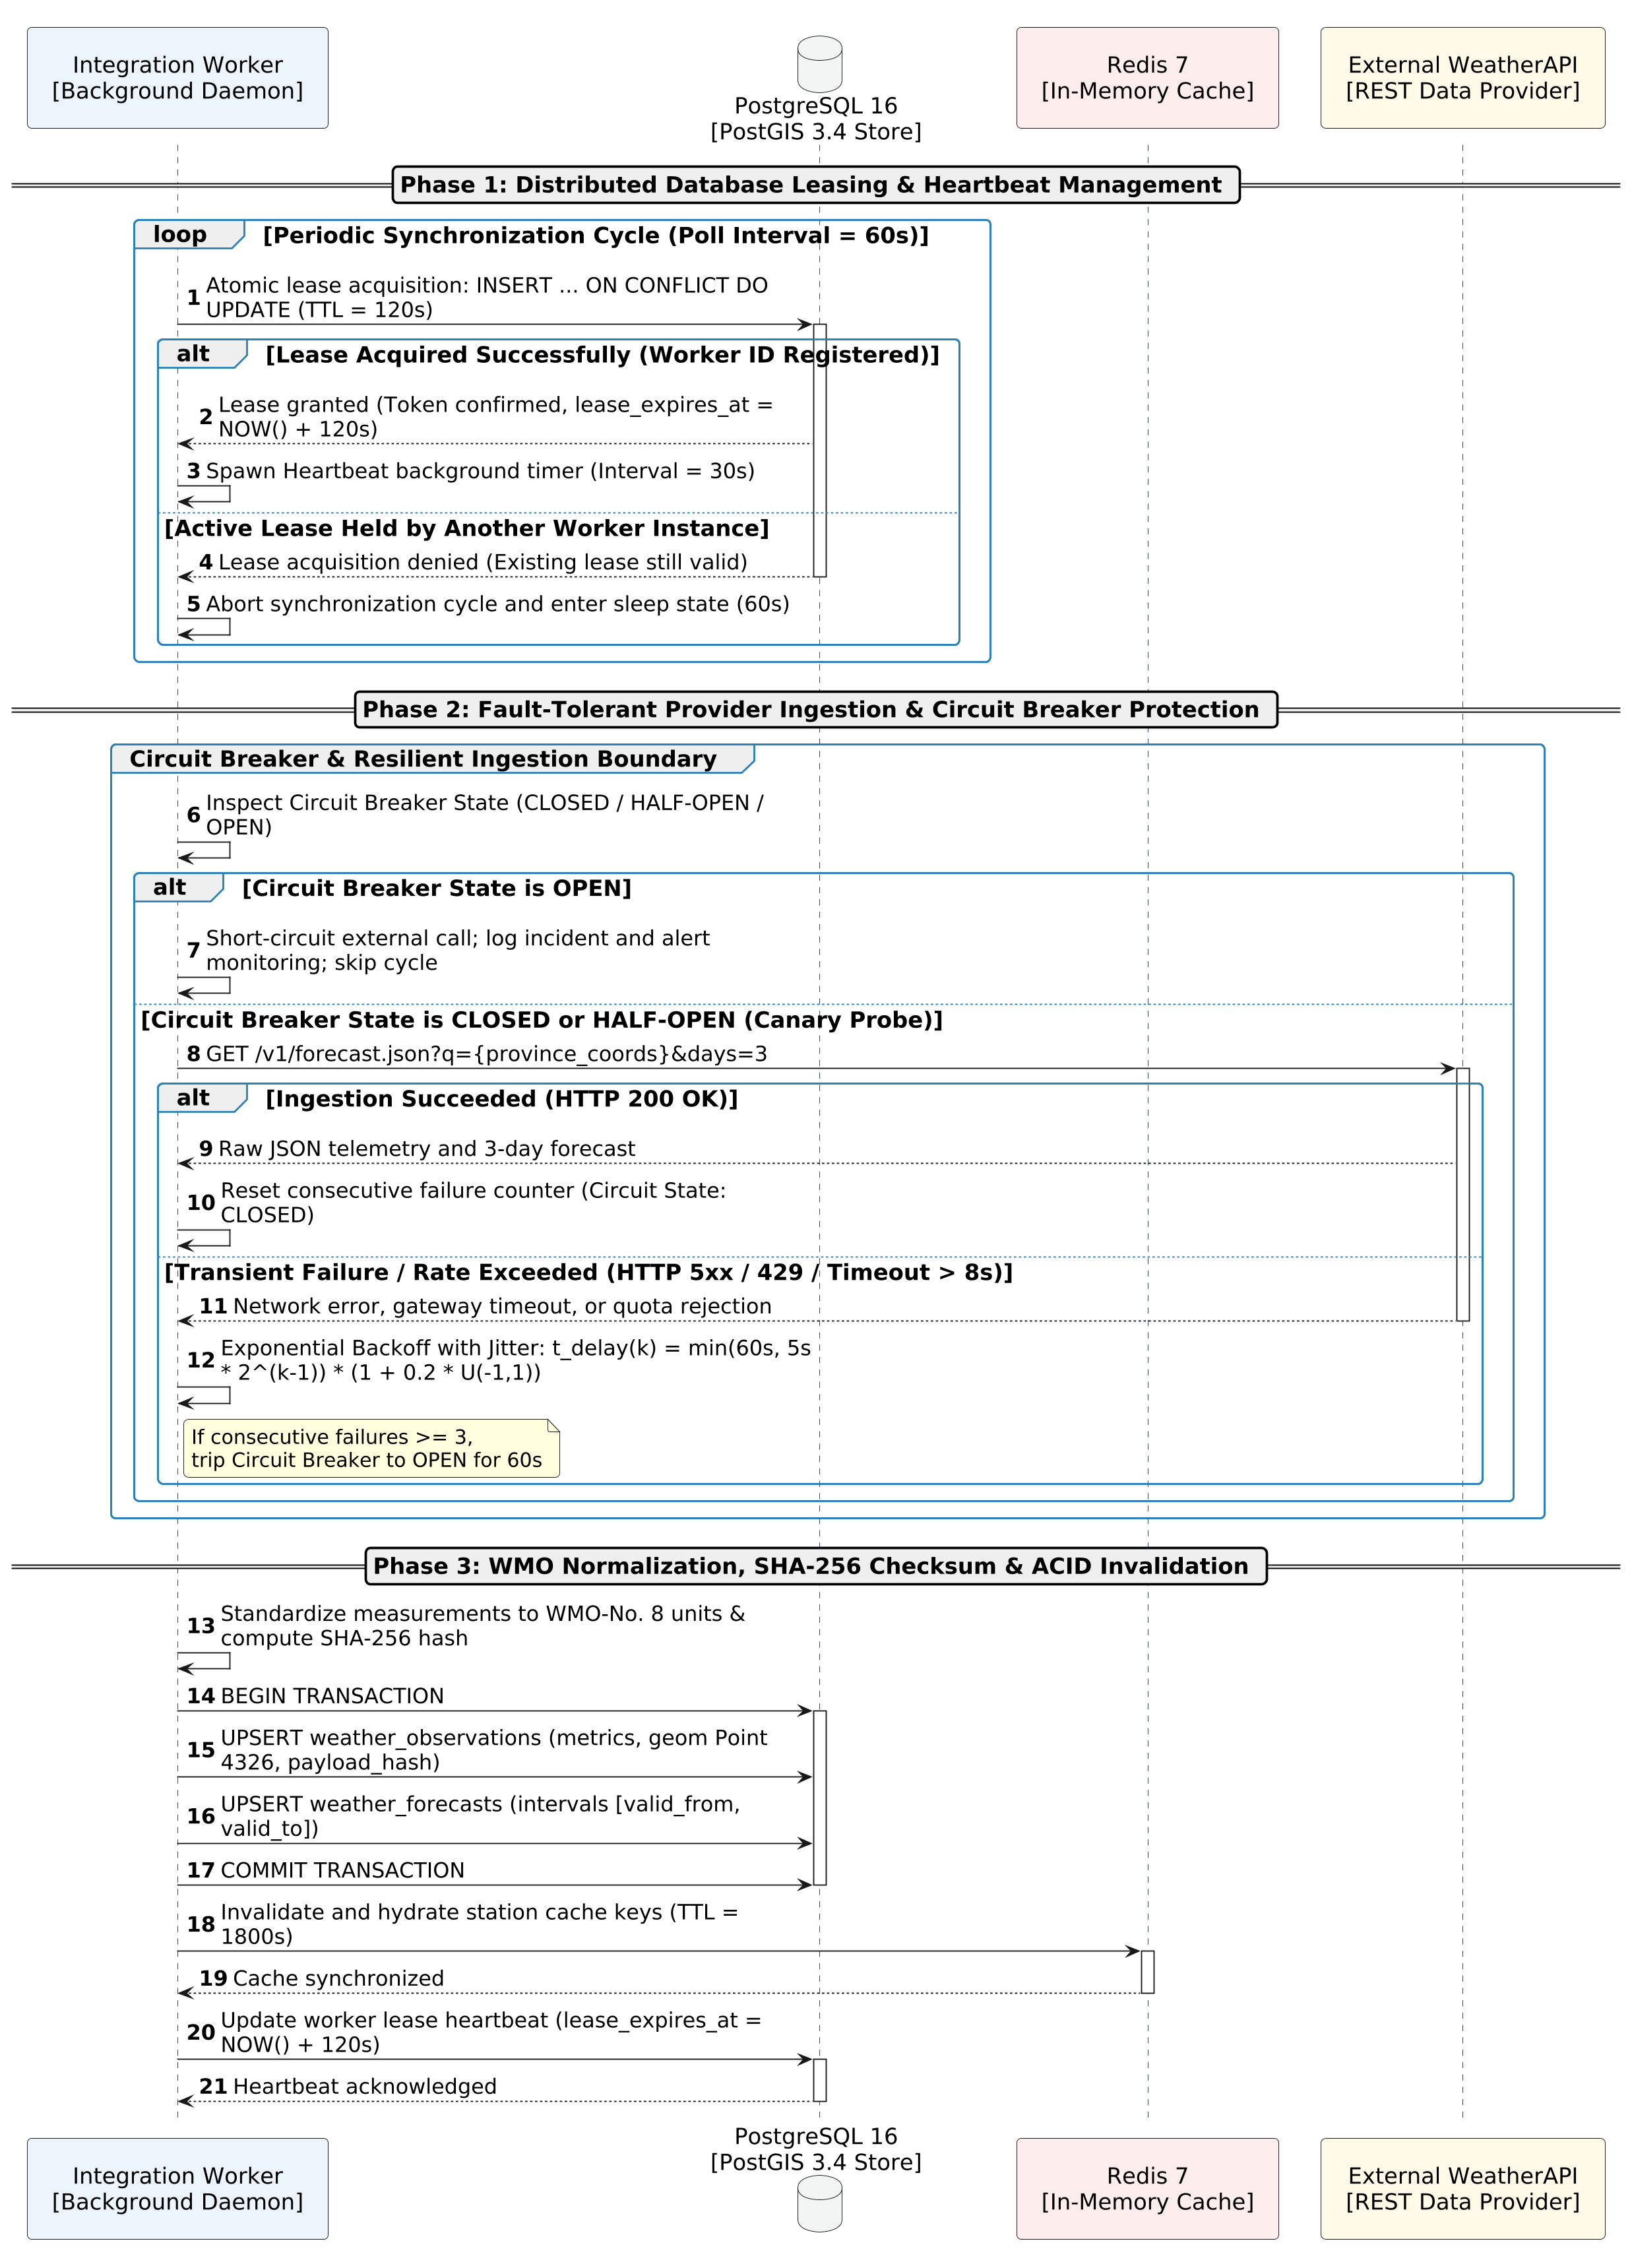
\includegraphics[width=0.92\textwidth, height=0.80\textheight, keepaspectratio]{figures/seq_ingestion.png}
\caption[Biểu đồ tuần tự đồng bộ dữ liệu thời tiết nền (ADR-001)]{Biểu đồ tuần tự quy trình đồng bộ dữ liệu khí tượng nền, cơ chế chiếm khóa phân tán và ngắt mạch tự động (ADR-001).}
\label{fig:seq_ingestion_vi}
\end{figure}

Flow hoạt động của tiến trình xử lý nền Integration Worker được phân rã thành ba giai đoạn vận hành then chốt:
\begin{itemize}
    \item[-] \textit{Pha 1: Chiếm khóa phân tán và quản trị nhịp tim (Distributed Database Leasing \& Heartbeat)}:
    Định kỳ mỗi 60 giây (chu kỳ thăm dò), worker phát câu lệnh kiểm tra và chiếm quyền độc quyền có thời hạn trên bảng \texttt{weather\_worker\_leases} của PostgreSQL thông qua lệnh nguyên tử \texttt{INSERT ... ON CONFLICT DO UPDATE WHERE lease\_expires\_at < NOW()}. Thao tác này bảo đảm chỉ duy nhất một tiến trình worker nắm giữ quyền thu thập dữ liệu trong cụm phân tán tại một thời điểm. Nếu chiếm khóa thành công (thời hạn giữ khóa $120.000\text{ ms}$), worker khởi tạo một bộ định thời nhịp tim (\texttt{heartbeat}) chạy ngầm với chu kỳ 30 giây để định kỳ cập nhật mốc thời gian hết hạn (\texttt{lease\_expires\_at} $= \text{NOW}() + 120\text{s}$). Ngược lại, nếu một tiến trình khác đang giữ khóa hợp lệ, yêu cầu bị từ chối và worker lập tức chuyển sang trạng thái ngủ trong 60 giây tiếp theo mà không gây xung đột tài nguyên.
    \item[-] \textit{Pha 2: Thu thập dữ liệu chịu lỗi và cơ chế ngắt mạch (Fault-Tolerant Provider Ingestion \& Circuit Breaker)}:
    Trước khi phát yêu cầu mạng tải dữ liệu 63 tỉnh thành, worker kiểm tra trạng thái của bộ ngắt mạch nội tại. Nếu mạch đang ở trạng thái Mở (\texttt{OPEN}), worker ngắn mạch ngay lập tức (short-circuit), hủy toàn bộ các cuộc gọi ra ngoài, ghi nhật ký cảnh báo và bỏ qua chu kỳ tải hiện tại. Nếu mạch ở trạng thái Đóng (\texttt{CLOSED}) hoặc Bán Mở (\texttt{HALF-OPEN}), worker gửi yêu cầu \texttt{GET /v1/forecast.json?q=\{province\_coords\}\&days=3} tới WeatherAPI. Khi nhận mã phản hồi HTTP 200 OK thành công, worker đặt lại bộ đếm lỗi liên tiếp về $0$. Trong trường hợp xảy ra lỗi nhất thời (mã lỗi HTTP 5xx, lỗi quá tải hạn ngạch HTTP 429 hoặc vượt quá thời gian chờ 8 giây), worker tính toán thời gian trì hoãn thử lại theo hàm số mũ kết hợp độ trễ ngẫu nhiên $t_{\text{delay}}(k)$ (Công thức~\eqref{eq:backoff_jitter}). Khi số lần thất bại liên tiếp đạt ngưỡng 3 lần, bộ ngắt mạch chuyển sang trạng thái \texttt{OPEN} trong 60 giây để bảo vệ hạn ngạch và tránh làm tê liệt dịch vụ đối tác.
    \item[-] \textit{Pha 3: Chuẩn hóa WMO, kiểm tra mã băm SHA-256 và giao dịch ACID (WMO Normalization, SHA-256 Checksum \& ACID Invalidation)}:
    Dữ liệu JSON thô nhận từ WeatherAPI được chuẩn hóa theo quy chuẩn khí tượng WMO-No. 8 (quy đổi nhiệt độ về độ C, tốc độ gió về mét/giây, lượng mưa về milimét). Worker sinh mã băm kiểm tra SHA-256 trên chuỗi dữ liệu chuẩn hóa để phát hiện các bản ghi trùng lặp nội dung. Tiếp theo, worker mở một khối giao dịch cơ sở dữ liệu (\texttt{BEGIN TRANSACTION}) và thực thi các câu lệnh \texttt{UPSERT} vào bảng \texttt{weather\_observations} (chứa các chỉ số quan trắc bề mặt kèm tọa độ hình học điểm \texttt{Point 4326}) và bảng \texttt{weather\_forecasts} (lưu trữ dự báo theo các khoảng thời gian hiệu lực), rồi xác nhận giao dịch (\texttt{COMMIT TRANSACTION}). Sau khi ghi dữ liệu bền vững thành công, worker phát tín hiệu làm mới và vô hiệu hóa bộ đệm Redis (\texttt{TTL = 1800s}) để các API phục vụ người dùng luôn đọc được dữ liệu mới nhất, đồng thời gửi tín hiệu nhịp tim cập nhật mốc thời gian khóa phân tán trong cơ sở dữ liệu.
\end{itemize}

\section{Mô hình Cơ sở Dữ liệu Không gian PostGIS và Lược đồ Thực thể (ERD)}
\label{sec:postgis_erd_schema}

\subsection{Cấu trúc Lược đồ Cơ sở Dữ liệu Phân tầng}
Cơ sở dữ liệu của hệ thống VietForecast được triển khai trên nền tảng PostgreSQL 16 tích hợp phần mở rộng không gian PostGIS 3.4. Lược đồ cơ sở dữ liệu được phân chia thành các nhóm miền dữ liệu chặt chẽ nhằm bảo đảm tính toàn vẹn tham chiếu và dễ dàng bảo trì:
\begin{itemize}
    \item[-] \textit{Nhóm an ninh phiên} (\texttt{app\_security}): Gồm bảng \texttt{app\_security.}\allowbreak\texttt{sessions} lưu trữ bản mã hóa AES-256-GCM của JWT, thẻ xác thực, thời điểm hết hạn và trạng thái thu hồi; bảng \texttt{app\_security.audit\_events} ghi nhận nhật ký bất biến về mọi hành vi truy cập nhạy cảm phục vụ kiểm toán an ninh.
    \item[-] \textit{Nhóm đơn vị hành chính và địa điểm} (\texttt{administrative}): Gồm bảng \texttt{administrative\_}\allowbreak\texttt{units} mô tả cấu trúc cây phân cấp hành chính lãnh thổ Việt Nam (Quốc gia $\rightarrow$ 63 Tỉnh/Thành phố $\rightarrow$ Quận/Huyện $\rightarrow$ Phường/Xã) kèm trường hình học \texttt{MultiPolygon}; bảng \texttt{locations} lưu trữ danh mục các điểm quan trắc, danh lam thắng cảnh và nút giao thông trọng yếu kèm tọa độ điểm \texttt{geometry(Point, 4326)}.
    \item[-] \textit{Nhóm dữ liệu khí tượng} (\texttt{weather}): Gồm bảng \texttt{weather\_providers} quản lý danh mục nhà cung cấp dữ liệu; bảng \texttt{weather\_observations} lưu trữ chuỗi thời gian các thông số quan trắc bề mặt thực nghiệm (nhiệt độ, lượng mưa, tốc độ gió, gió giật, tầm nhìn, mã WMO, giá trị băm kiểm tra SHA-256); bảng \texttt{weather\_forecasts} lưu trữ dự báo thời tiết theo các khoảng hiệu lực $[t_{\text{start}}, t_{\text{end}}]$; và bảng \texttt{weather\_worker\_leases} điều phối khóa phân tán.
    \item[-] \textit{Nhóm quy tắc rủi ro và đánh giá lộ trình} (\texttt{risk\_route}): Gồm các bảng \texttt{risk\_}\allowbreak\texttt{rule\_}\allowbreak\texttt{sets} và \texttt{risk\_}\allowbreak\texttt{rules} lưu trữ các ngưỡng tham số khí tượng theo từng loại phương tiện dưới cơ chế quản trị đa cấp (Maker-Checker); bảng \texttt{risk\_}\allowbreak\texttt{assessments} và \texttt{risk\_}\allowbreak\texttt{assessment\_}\allowbreak\texttt{evidence} lưu vết kết quả đánh giá cùng bằng chứng quan trắc phục vụ kiểm toán; các bảng \texttt{route\_}\allowbreak\texttt{requests}, \texttt{route\_}\allowbreak\texttt{options} và \texttt{route\_}\allowbreak\texttt{samples} lưu trữ yêu cầu tìm đường, hình học đa tuyến LineString của các lộ trình thay thế và các điểm lấy mẫu không-thời gian dọc tuyến.
\end{itemize}

\subsection{Tối ưu hóa Truy vấn Không gian với Cây Chỉ mục GiST}
Trong bài toán đánh giá rủi ro tuyến đường, hệ thống cần truy vấn toàn bộ các trạm thời tiết nằm trong hành lang đệm có bán kính $r_{\text{corridor}} = 15\text{ km}$ bao quanh một lộ trình di chuyển trải dài hàng trăm kilômét (tương ứng với hàng nghìn điểm tọa độ). Nếu thực hiện tính toán khoảng cách cầu phẳng trực tiếp bằng phép quét toàn bảng (Sequential Scan), độ phức tạp thuật toán sẽ đạt mức $O(M \cdot N)$ (với $M$ là số điểm lấy mẫu trên lộ trình và $N$ là tổng số trạm thời tiết), dẫn đến thời gian phản hồi kéo dài hàng giây và làm quá tải tài nguyên máy chủ.

Để giải quyết triệt để vấn đề này, PostGIS 3.4 kích hoạt cây chỉ mục tìm kiếm tổng quát GiST (Generalized Search Tree) trên toàn bộ các cột kiểu hình học \texttt{geom}. Cây chỉ mục GiST tổ chức các phần tử không gian dưới dạng cây phân cấp các hộp chữ nhật bao tối thiểu (Minimum Bounding Box -- BBOX). Động cơ cơ sở dữ liệu áp dụng quy trình lọc hai giai đoạn (Two-Tier Spatial Filtering):
\begin{itemize}
    \item[-] \textit{Giai đoạn lọc thô (Rough Pass - Bounding Box Filter)}: Hệ thống kiểm tra điều kiện giao cắt giữa hộp bao của hành lang đệm tuyến đường $G_{\text{corridor}} = \text{ST\_Buffer}(\mathcal{L}, r_{\text{corridor}})$ và hộp bao của từng điểm quan trắc:
    \begin{equation}
    \label{eq:spatial_bbox_filter_vi}
    \text{BBOX}(o.\text{geom}) \cap \text{BBOX}(G_{\text{corridor}}) \ne \emptyset
    \end{equation}
    Nhờ cấu trúc cây cân bằng của GiST, độ phức tạp của giai đoạn này chỉ là $O(\log N)$, loại bỏ hơn 95\% các trạm quan trắc nằm ngoài phạm vi tiềm năng mà không cần tính toán tọa độ chi tiết.
    \item[-] \textit{Giai đoạn lọc tinh (Exact Pass)}: Động cơ PostGIS chỉ áp dụng công thức hình học cầu trắc địa phức tạp (hàm \texttt{ST\_DWithin} trên kiểu dữ liệu \texttt{geography}) đối với tập hợp các trạm đã vượt qua giai đoạn lọc thô:
    \begin{equation}
    \label{eq:spatial_exact_filter_vi}
    d_{\text{geodetic}}(o.\text{geom}, \mathcal{L}) \le r_{\text{corridor}} \quad \text{với } \tau(o) \le 180\text{ phút}
    \end{equation}
    bảo đảm kết quả chính xác tuyệt đối theo độ cong elipxoit WGS84 với thời gian phản hồi ở mức dưới 15 mili-giây. Chi tiết thông số khai báo chỉ mục GiST và đặc tả truy vấn không gian tối ưu được trình bày trong Bảng~\ref{tab:gist_query_spec_vi} tại Chương~\ref{ch:implementation}.
\end{itemize}

\subsection{Lược đồ Thực thể Quan hệ Chuẩn hóa (ERD) và Cơ chế Quản trị Dữ liệu}
Hình~\ref{fig:erd_database_vi} biểu diễn lược đồ quan hệ thực thể (Entity-Relationship Diagram -- ERD) giữa các bảng dữ liệu then chốt trong hệ thống VietForecast, thể hiện các khóa chính, khóa ngoại và ràng buộc toàn vẹn dữ liệu.

\begin{figure}[H]
\centering
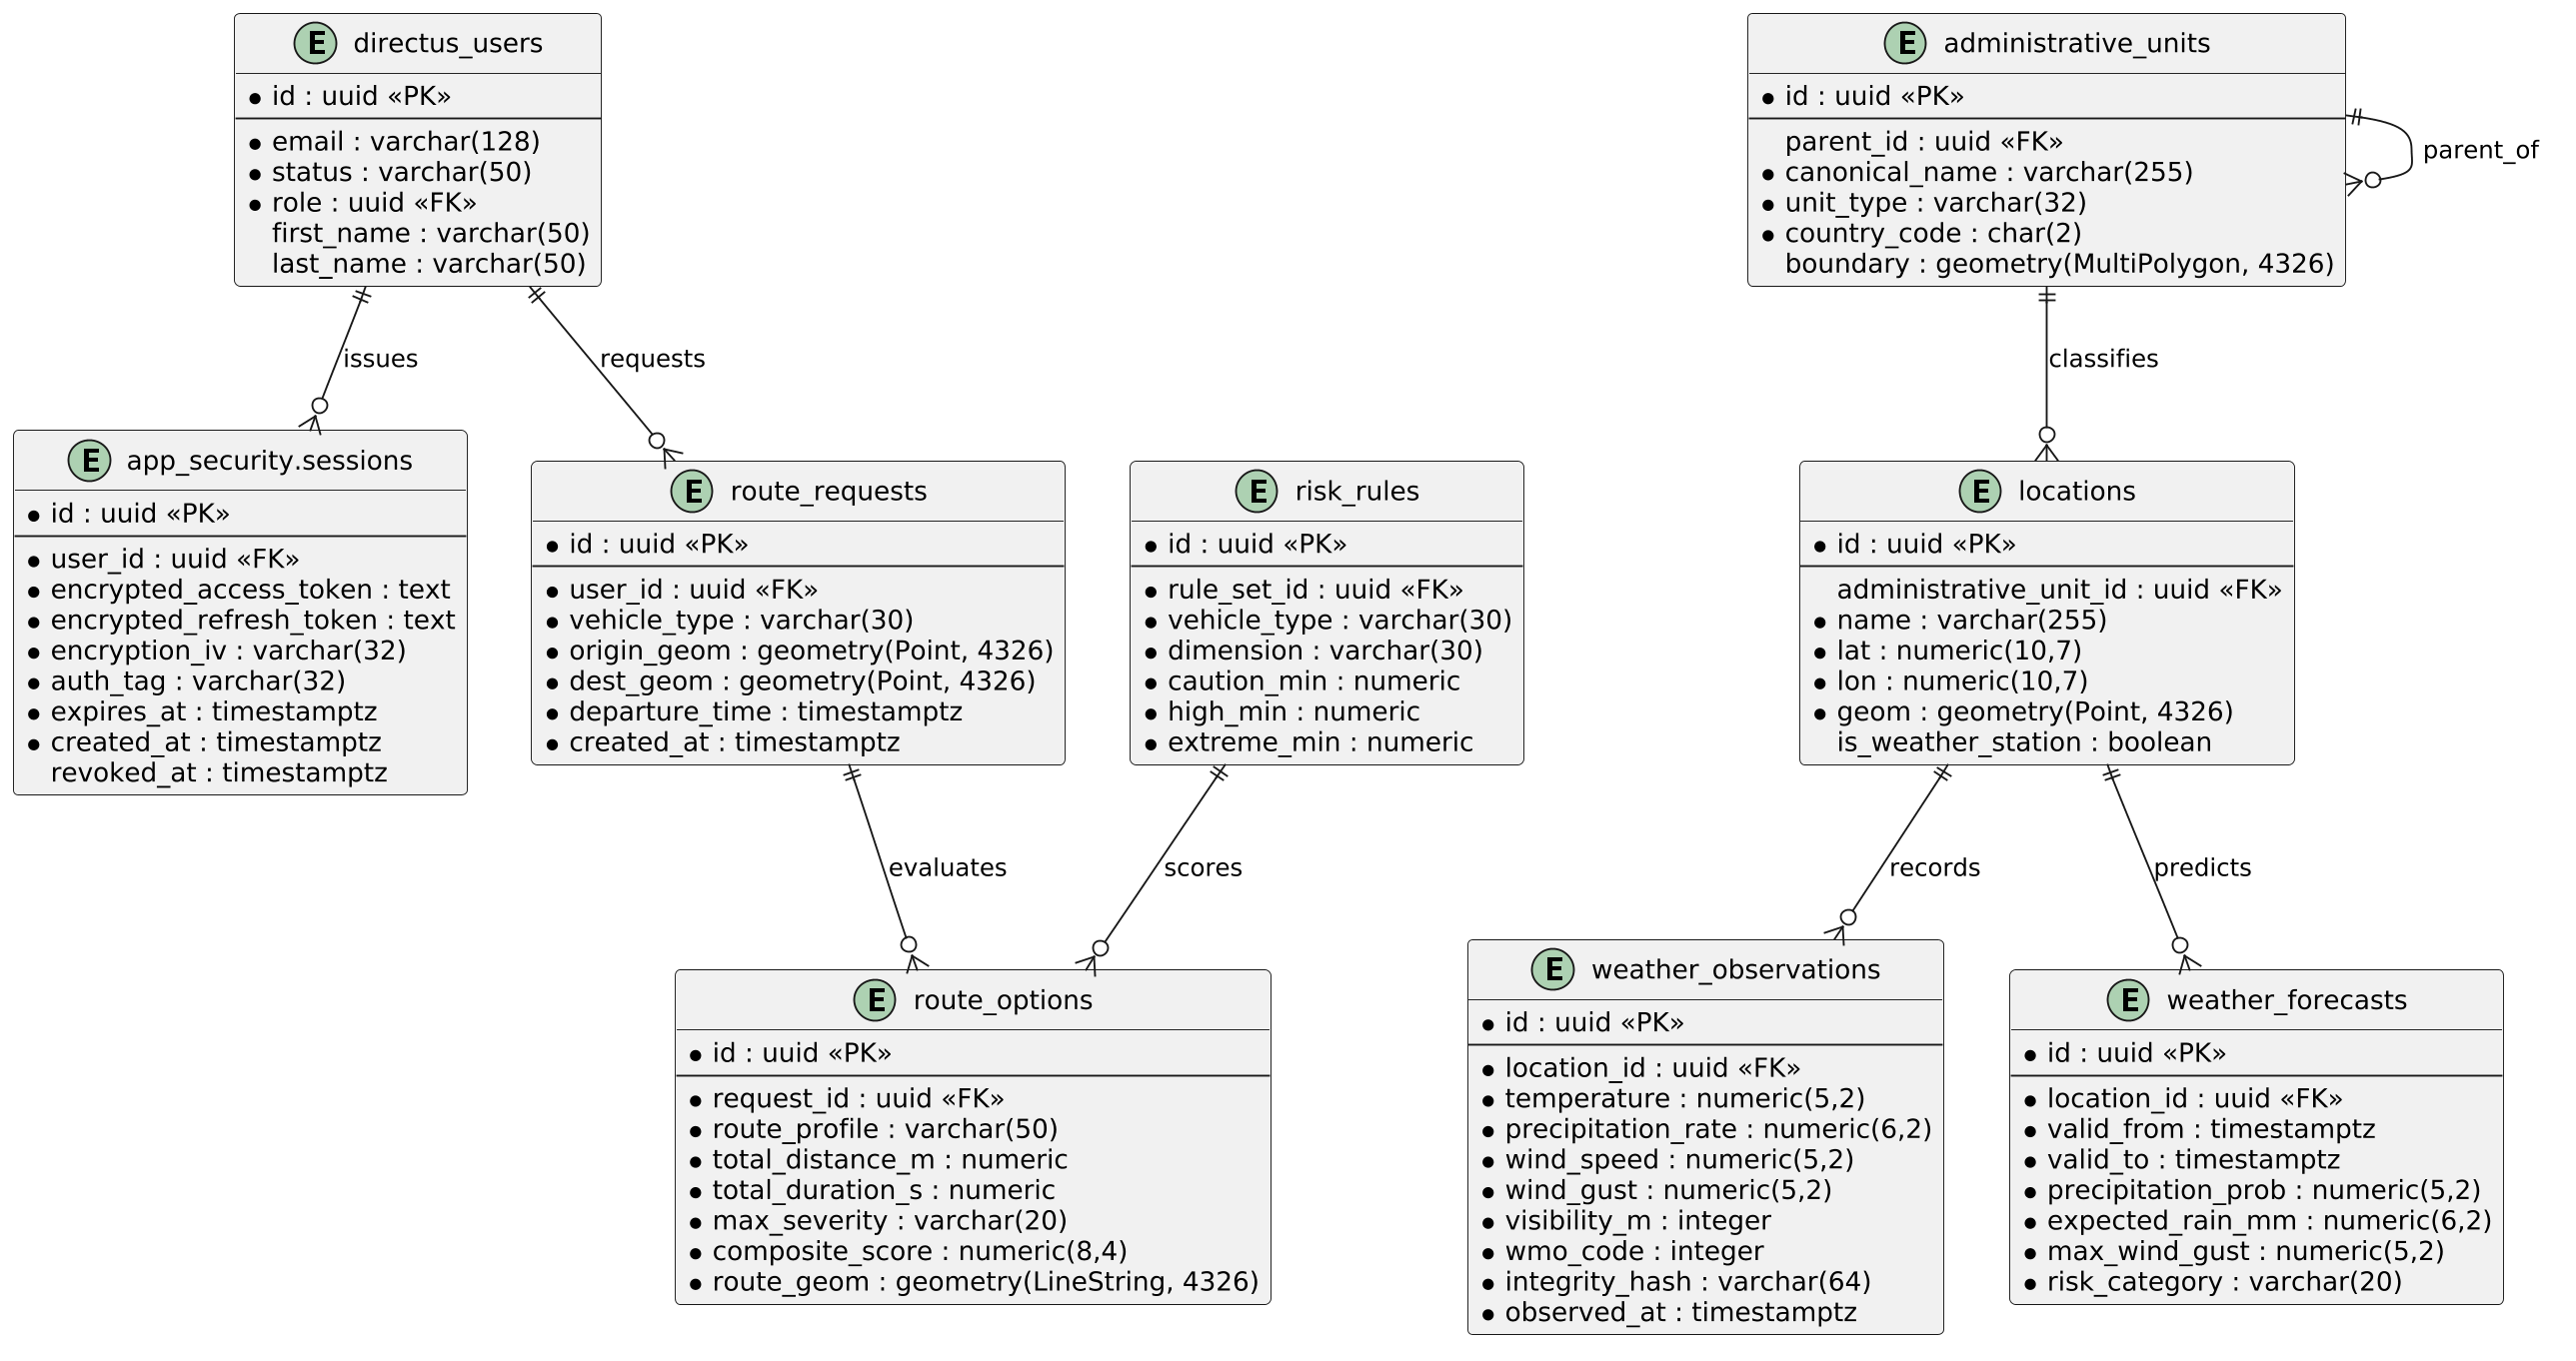
\includegraphics[width=0.95\textwidth, height=0.62\textheight, keepaspectratio]{figures/erd_database.png}
\caption[Lược đồ Thực thể Quan hệ (ERD) VietForecast]{Lược đồ Thực thể Quan hệ (ERD) mô tả cấu trúc dữ liệu không gian, an ninh danh tính và quy tắc rủi ro của VietForecast.}
\label{fig:erd_database_vi}
\end{figure}

Trong lược đồ thực thể, thực thể người dùng \texttt{directus\_}\allowbreak\texttt{users} đóng vai trò là điểm neo định danh duy nhất cho toàn bộ hệ sinh thái, vừa phát hành các phiên làm việc bảo mật trong \texttt{app\_}\allowbreak\texttt{security.}\allowbreak\texttt{sessions}, vừa liên kết với lịch sử các yêu cầu định tuyến trong \texttt{route\_}\allowbreak\texttt{requests}. Mô hình dữ liệu áp dụng hai cơ chế quản trị toàn vẹn chuyên sâu:
\begin{itemize}
    \item[-] \textit{Cơ chế kiểm soát phát hành quy tắc rủi ro (Maker-Checker Governance)}: Bộ quy tắc rủi ro trong bảng \texttt{risk\_}\allowbreak\texttt{rule\_}\allowbreak\texttt{sets} vận hành theo máy trạng thái tuần tự bao gồm các nấc: \texttt{draft}, \texttt{review}, \texttt{approved}, \texttt{published} và \texttt{retired}. Trigger cơ sở dữ liệu \texttt{app\_}\allowbreak\texttt{governance.}\allowbreak\texttt{guard\_}\allowbreak\texttt{risk\_}\allowbreak\texttt{rule\_}\allowbreak\texttt{mutation()} lập tức chặn đứng mọi hành vi chỉnh sửa hoặc xóa bỏ bản ghi con trong \texttt{risk\_}\allowbreak\texttt{rules} một khi tập quy tắc đã chuyển trạng thái rời khỏi \texttt{draft}, bảo đảm tính tất định và bất biến của các phán quyết rủi ro trong quá khứ.
    \item[-] \textit{Nhật ký kiểm toán an ninh bất biến (Immutable Audit Trail)}: Toàn bộ các thao tác nhạy cảm liên quan đến danh tính, phân quyền và điều chỉnh ngưỡng khí tượng đều kích hoạt ghi nhận vào bảng nhật ký kiểm toán \texttt{app\_}\allowbreak\texttt{security.}\allowbreak\texttt{audit\_}\allowbreak\texttt{events}. Quyền ghi nhật ký được cấp tự động thông qua hàm trigger chạy với quyền hạn bảo mật (\texttt{SECURITY DEFINER}), ngăn chặn hoàn toàn khả năng người dùng hoặc tiến trình ứng dụng can thiệp nhằm che giấu vết tích xâm nhập.
\end{itemize}

\section{Thiết kế Động cơ Đánh giá Rủi ro và Lập Lộ trình Cân bằng Đa Mục tiêu}
\label{sec:route_risk_engine}

\subsection{Mô hình Không-Thời gian và Rời rạc hóa Hành lang Di chuyển}
Động cơ đánh giá rủi ro tuyến đường của VietForecast được thiết kế nhằm giải quyết bài toán cốt lõi: biến các dữ liệu khí tượng rời rạc từ các trạm quan trắc thành chỉ dẫn di chuyển có thể hành động được cho người điều khiển phương tiện trên đường.

Hệ thống tiếp nhận các phương án lộ trình từ dịch vụ định tuyến đường bộ (OSRM), bao gồm: tuyến nhanh nhất (Fastest), tuyến ngắn nhất (Shortest) và tuyến thay thế (Alternative), mỗi tuyến biểu diễn dưới dạng đa tuyến GeoJSON LineString kèm thông số cự ly tổng $D$ và thời gian di chuyển danh định $T$. Với từng phương án lộ trình, động cơ phân rã đa tuyến thành dãy các điểm kiểm tra $p_i = (\phi_i, \lambda_i)$ với hai ràng buộc giới hạn: khoảng cách không gian giữa hai điểm liên tiếp $\Delta s \le 5\text{ km}$ và chênh lệch thời gian tiếp cận $\Delta t \le 15\text{ phút}$, tính toán dựa trên vận tốc danh định trung bình $\bar{v} = D / T$.

Fastify API thực thi truy vấn PostGIS với hàm \texttt{ST\_DWithin} để tìm kiếm các trạm quan trắc hoặc lưới dự báo thời tiết nằm trong hành lang đệm 15 km quanh từng điểm $p_i$, gán trường khí tượng tương ứng tại mốc thời gian ước lượng $t_i$.

\subsection{Ma trận Ngưỡng Rủi ro Phân hóa Phương tiện}
Động cơ rủi ro đối chiếu các tham số khí tượng tại từng điểm $p_i$ với tập luật rủi ro sáu chiều ($R_{\text{rain}}$, $R_{\text{wind}}$, $R_{\text{temp}}$, $R_{\text{vis}}$, $R_{\text{storm}}$, $R_{\text{alert}}$). Cấp độ rủi ro tại mỗi điểm lấy mẫu $S(p_i)$ tuân theo quy tắc rủi ro bao trùm nghiêm trọng nhất (Max-Severity Aggregation):
\begin{equation}
\label{eq:max_severity_aggregation_vi}
S(p_i) = \max_{d \in \mathcal{D}} R_d(p_i, v)
\end{equation}
trong đó $\mathcal{D} = \{\text{rain}, \text{wind}, \text{temp}, \text{vis}, \text{storm}, \text{alert}\}$ là tập 6 chiều rủi ro khí tượng, $v \in \{\text{motorcycle}, \text{car}\}$ biểu thị loại phương tiện tham gia giao thông, và $R_d \in \{0, 1, 2, 3\}$ tương ứng với 4 cấp độ: \texttt{Unknown} (0), \texttt{Low} (1), \texttt{Caution} (2), và \texttt{High} (3).

Bảng~\ref{tab:vehicle_risk_matrix_vi} chi tiết hóa ma trận ngưỡng kích hoạt rủi ro phân hóa theo phương tiện theo quy chuẩn an toàn giao thông đường bộ Việt Nam.

\begin{table}[H]
\centering
\small
\caption[Ma trận ngưỡng rủi ro phân hóa theo loại phương tiện]{Ma trận ngưỡng kích hoạt rủi ro thời tiết phân hóa theo loại phương tiện (RISK-001, RISK-002).}
\label{tab:vehicle_risk_matrix_vi}
\begin{tabularx}{\textwidth}{l >{\raggedright\arraybackslash}p{2.8cm} X X}
\toprule
\textbf{Chiều rủi ro} & \textbf{Chỉ số \& Đơn vị} & \textbf{Ngưỡng Thận trọng (Caution)} & \textbf{Ngưỡng Nguy hiểm (High)} \\
\midrule
Lượng mưa ($R_{\text{rain}}$) & Cường độ mưa (mm/h) & 
Xe máy: $10 \le r < 25$ \newline Ô tô: $15 \le r < 35$ & 
Xe máy: $r \ge 25$ \newline Ô tô: $r \ge 35$ \\
\addlinespace
Gió giật ($R_{\text{wind}}$) & Vận tốc gió giật (km/h) & 
Xe máy: $25 \le w < 40$ \newline Ô tô: $45 \le w < 60$ & 
Xe máy: $w \ge 40$ \newline Ô tô: $w \ge 60$ \\
\addlinespace
Tầm nhìn ($R_{\text{vis}}$) & Tầm nhìn ngang (m) & 
Xe máy: $1.000 \le v < 2.000$ \newline Ô tô: $500 \le v < 1.000$ & 
Xe máy: $v < 1.000$ \newline Ô tô: $v < 500$ \\
\addlinespace
Nhiệt độ ($R_{\text{temp}}$) & Nhiệt độ bề mặt ($^\circ\text{C}$) & 
Xe máy: $36$--$38^\circ\text{C}$ hoặc $10$--$13^\circ\text{C}$ \newline Ô tô: $38$--$40^\circ\text{C}$ hoặc $5$--$8^\circ\text{C}$ & 
Xe máy: $> 38^\circ\text{C}$ hoặc $< 10^\circ\text{C}$ \newline Ô tô: $> 40^\circ\text{C}$ hoặc $< 5^\circ\text{C}$ \\
\addlinespace
Dông sét ($R_{\text{storm}}$) & Hiện tượng đối lưu WMO & 
Có dông xa hoặc mây vũ tích & 
Dông sét trực tiếp hoặc mưa đá \\
\addlinespace
Cảnh báo ($R_{\text{alert}}$) & Cấp thiên tai quốc gia & 
Rủi ro thiên tai Cấp 1--2 & 
Rủi ro thiên tai Cấp 3 trở lên \\
\bottomrule
\end{tabularx}
\end{table}

\subsection{Hàm Mục tiêu Tối ưu hóa Cân bằng Tuyến đường}
Hệ thống tính toán điểm số tổng hợp cho từng phương án lộ trình dựa trên công thức hàm mục tiêu chuẩn hóa:
\begin{equation}
\label{eq:route_balanced_score_vi}
Score_{\text{balanced}} = w_{\text{risk}} \cdot \hat{S}_{\text{route}} + w_{\text{time}} \cdot \hat{T} + w_{\text{dist}} \cdot \hat{D}
\end{equation}
với bộ trọng số mặc định $w_{\text{risk}} = 0{,}5$, $w_{\text{time}} = 0{,}3$, $w_{\text{dist}} = 0{,}2$. Điểm rủi ro trung bình dọc tuyến $\hat{S}_{\text{route}} = \frac{1}{K} \sum_{k=1}^K S(p_k) / 3$, cự ly $\hat{D} = D / \max(D)$ và thời gian $\hat{T} = T / \max(T)$ được chuẩn hóa về miền $[0, 1]$. Tuyến đường có điểm số thấp nhất sẽ được gắn nhãn Khuyến nghị an toàn (Weather-Safer Recommended), giúp người lái xe cân bằng tối ưu giữa thời gian hành trình và sự an toàn tính mạng trước các hình thái thời tiết cực đoan.

\subsection{Quy trình Đánh giá Rủi ro Lộ trình và Biểu đồ Tuần tự}
Hình~\ref{fig:seq_route_risk_vi} mô tả chi tiết biểu đồ tuần tự toàn diện của luồng đánh giá rủi ro thời tiết lộ trình đa phương án từ khi người dùng phát lệnh tìm đường trên giao diện MapLibre GL.

\begin{figure}[H]
\centering
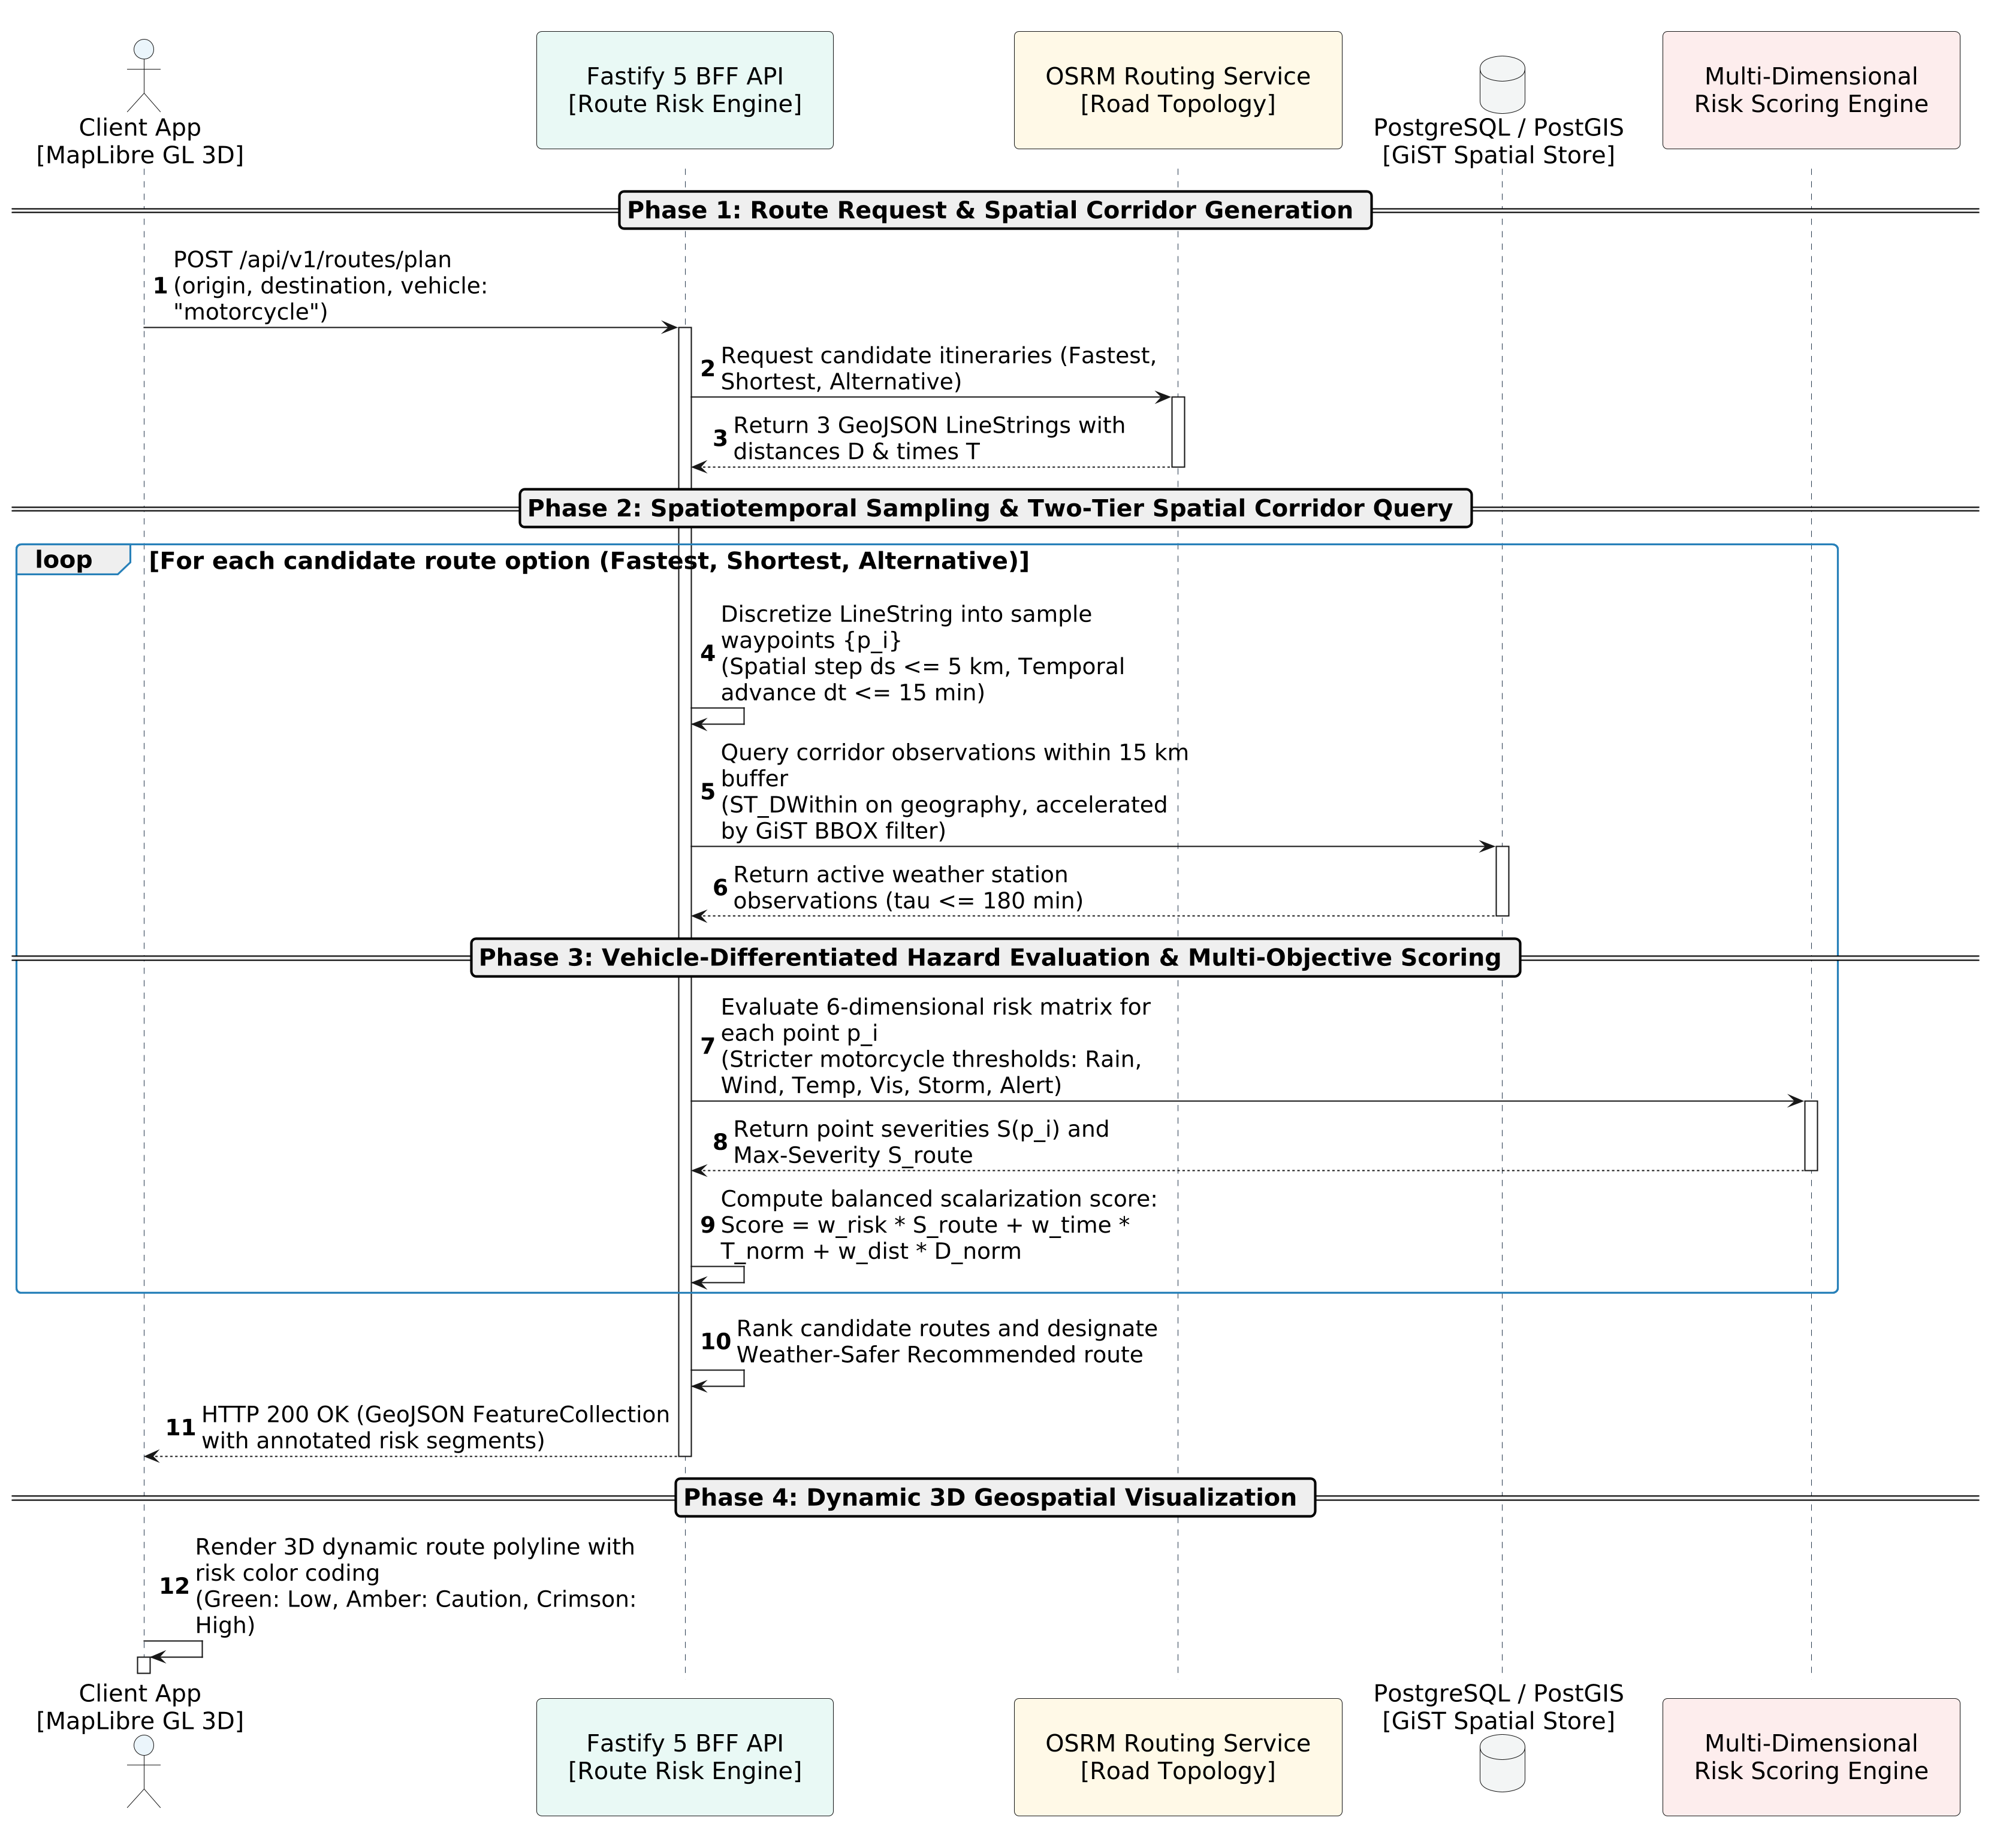
\includegraphics[width=0.95\textwidth, keepaspectratio]{figures/seq_route_risk.png}
\caption[Biểu đồ tuần tự đánh giá rủi ro thời tiết lộ trình]{Biểu đồ tuần tự quy trình đánh giá rủi ro thời tiết lộ trình đa mục tiêu, lấy mẫu không-thời gian và trực quan hóa bản đồ 3D.}
\label{fig:seq_route_risk_vi}
\end{figure}

Flow hoạt động của quy trình đánh giá rủi ro lộ trình bao gồm bốn pha chính xác như sau:
\begin{itemize}
    \item[-] \textit{Pha 1: Tiếp nhận yêu cầu tìm đường và khai phá lộ trình ứng viên}:
    Ứng dụng khách MapLibre GL gửi yêu cầu \texttt{POST /api/v1/routes/plan} kèm tọa độ điểm xuất phát, điểm đến và loại phương tiện (\texttt{motorcycle} hoặc \texttt{car}) tới Fastify API. Fastify chuyển tiếp yêu cầu tới dịch vụ định tuyến đường bộ OSRM để thu nhận ba phương án lộ trình độc lập: tuyến nhanh nhất (Fastest), tuyến ngắn nhất (Shortest) và tuyến thay thế (Alternative). Mỗi tuyến được định nghĩa dưới dạng đa tuyến hình học GeoJSON LineString kèm các thông số cự ly tổng $D$ và thời gian di chuyển danh định $T$.
    \item[-] \textit{Pha 2: Rời rạc hóa không-thời gian và truy vấn trắc địa hành lang đệm}:
    Với từng phương án lộ trình, động cơ phân rã đa tuyến LineString thành dãy các điểm kiểm tra $p_i = (\phi_i, \lambda_i)$ với hai ràng buộc giới hạn: khoảng cách không gian giữa hai điểm liên tiếp $\Delta s \le 5\text{ km}$ và chênh lệch thời gian tiếp cận $\Delta t \le 15\text{ phút}$ (tính dựa trên vận tốc danh định trung bình $\bar{v} = D / T$).
    Tại từng điểm kiểm tra $p_i$, Fastify API thực thi truy vấn không gian trắc địa PostGIS thông qua hàm \texttt{ST\_DWithin}. Nhờ cây chỉ mục GiST 2D, hệ thống thực hiện phép lọc thô qua hộp bao BBOX với độ phức tạp chỉ $O(\log N)$, sau đó mới tính toán cự ly trắc địa elipxoit WGS84 chính xác để thu thập toàn bộ các trạm quan trắc hoặc lưới dự báo trong hành lang đệm bán kính $r_{\text{corridor}} = 15\text{ km}$ có độ tươi mới dữ liệu $\tau \le 180\text{ phút}$.
    \item[-] \textit{Pha 3: Đánh giá ma trận rủi ro phân hóa phương tiện và chấm điểm đa mục tiêu}:
    Động cơ đối chiếu các thông số quan trắc khí tượng thu nhận được tại từng điểm $p_i$ với tập luật rủi ro sáu chiều: Lượng mưa ($R_{\text{rain}}$), Gió giật ($R_{\text{wind}}$), Nhiệt độ ($R_{\text{temp}}$), Tầm nhìn ($R_{\text{vis}}$), Dông sét ($R_{\text{storm}}$) và Cấp độ thiên tai ($R_{\text{alert}}$). Cấp độ rủi ro tại mỗi điểm $S(p_i)$ tuân theo quy tắc bao trùm nghiêm trọng nhất $S(p_i) = \max_{d \in \mathcal{D}} R_d(p_i, v)$ theo công thức~\eqref{eq:max_severity_aggregation_vi}. Đối với xe máy, các ngưỡng kích hoạt được siết chặt hơn 30\% so với ô tô nhằm phản ánh nguy cơ mất an toàn thực tế (Bảng~\ref{tab:vehicle_risk_matrix_vi}).
    Hệ thống tính toán điểm số hàm mục tiêu cân bằng $Score_{\text{balanced}}$ theo công thức~\eqref{eq:route_balanced_score_vi}, kết hợp giữa độ an toàn thời tiết dọc tuyến ($\hat{S}_{\text{route}}$), thời gian di chuyển ($\hat{T}$) và cự ly hành trình ($\hat{D}$). Tuyến đường có điểm số tổng hợp thấp nhất được xếp hạng ưu tiên và gắn nhãn Khuyến nghị an toàn (Weather-Safer Recommended).
    \item[-] \textit{Pha 4: Đóng gói dữ liệu và trực quan hóa 3D động}:
    Fastify API hoàn tất tính toán và trả về phản hồi HTTP 200 OK dưới dạng gói GeoJSON FeatureCollection chứa các đa tuyến lộ trình đã phân đoạn và gắn mã màu rủi ro tương ứng: xanh lục (\texttt{Low}), vàng cam (\texttt{Caution}) và đỏ thẫm (\texttt{High}). Ứng dụng giao diện MapLibre GL 4 tận dụng khả năng tăng tốc phần cứng WebGL để dựng mô hình địa hình ba chiều (3D terrain), hiển thị đa tuyến lộ trình động và cho phép người lái xe trực tiếp theo dõi các phân đoạn nguy hiểm dọc hành trình.
\end{itemize}

\section{Thiết kế Trợ lý AI Khí tượng Đàm thoại có Kiểm chứng Dữ liệu}
\label{sec:grounded_ai_assistant}

\subsection{Kiến trúc Điều phối Công cụ Đàm thoại (Tool Orchestration)}
Để đáp ứng nhu cầu giao tiếp đàm thoại tự nhiên của người dùng mà vẫn kiểm soát và giảm thiểu tối đa hiện tượng ảo giác (hallucination) thường gặp ở các mô hình ngôn ngữ lớn, VietForecast thiết kế kiến trúc Trợ lý AI có kiểm chứng dữ liệu thực nghiệm (Grounded AI Engine) dựa trên mô hình nền tảng Google Gemini 1.5 Flash.

Google Gemini 1.5 Flash được cấu hình đóng vai trò là bộ phân tích ngôn ngữ tự nhiên và điều phối công cụ (Tool Orchestrator). Mô hình hoàn toàn không được phép tự do tạo sinh các thông số khí tượng giả lập. Hệ thống trang bị cho Gemini năm công cụ gọi hàm chuẩn hóa:
\begin{itemize}
    \item[-] \texttt{search\_location}: Tra cứu tọa độ, đơn vị hành chính và địa danh từ cơ sở dữ liệu chuẩn hóa 63 tỉnh thành.
    \item[-] \texttt{get\_current\_weather}: Trích xuất các thông số quan trắc khí tượng bề mặt mới nhất tại trạm đo tương ứng.
    \item[-] \texttt{get\_forecast}: Lấy chuỗi dữ liệu dự báo khí quyển theo từng khoảng hiệu lực thời gian.
    \item[-] \texttt{assess\_travel\_risk}: Tính toán cấp độ rủi ro tại một địa điểm cụ thể dựa trên ma trận ngưỡng phương tiện.
    \item[-] \texttt{evaluate\_route}: Đánh giá an toàn lộ trình qua hàm ánh xạ:
    \begin{equation}
    \label{eq:tool_evaluate_route_vi}
    \mathcal{F}_{\text{route}}: (\text{origin}, \text{destination}, \text{vehicleType}) \longrightarrow \text{RouteRiskAssessment}
    \end{equation}
    Khai báo đặc tả tham số chi tiết của công cụ gọi hàm \texttt{evaluate\_route} được trình bày trong Bảng~\ref{tab:gemini_tool_schema_vi} tại Chương~\ref{ch:implementation}.
\end{itemize}

\subsection{Cơ chế Kiểm chứng Dữ liệu và Trích dẫn Thực nghiệm (Grounded Evidence Pipeline)}
Chu trình kiểm chứng dữ liệu thực nghiệm vận hành theo ba bước nghiêm ngặt:
\begin{itemize}
    \item[-] \textit{Tiếp nhận và gọi công cụ}: Khi nhận diện câu hỏi từ người dùng (ví dụ: \textit{"Chiều nay tôi đi xe máy từ Hà Nội về Ninh Bình có an toàn không?"}), Gemini sinh cấu trúc gọi công cụ \texttt{evaluate\_route}. Fastify API đón bắt lệnh gọi, thực thi truy vấn PostGIS và dịch vụ định tuyến, kiểm tra độ tươi mới $\tau \le 180\text{ phút}$, rồi đóng gói dữ liệu quan trắc thực tế gửi ngược lại mô hình.
    \item[-] \textit{Tổng hợp câu trả lời kèm bằng chứng}: Gemini tổng hợp câu trả lời bằng tiếng Việt tự nhiên dựa độc quyền trên dữ liệu được cung cấp. Phản hồi bắt buộc đính kèm trích dẫn nguồn trạm đo (Station ID), mốc thời gian quan trắc và câu khuyến cáo an toàn bắt buộc.
    \item[-] \textit{Cơ chế dự phòng tất định (Deterministic Fallback Engine)}: Trong trường hợp đường truyền quốc tế gián đoạn hoặc dịch vụ Gemini vượt hạn mức, bộ điều phối \texttt{GroundedRuleEngineAdapter} tại Fastify API tự động kích hoạt. Thành phần này dùng biểu thức chính quy (regular expressions) nhận dạng thực thể vị trí và áp dụng trực tiếp cây quyết định tất định để trả về kết quả dự báo và cảnh báo rủi ro chính xác 100\% mà không làm gián đoạn trải nghiệm người dùng.
\end{itemize}

\section{Tóm tắt chương}
\label{sec:chapter3_summary}
Chương 3 đã trình bày chi tiết toàn bộ thiết kế kiến trúc hệ thống và thiết kế kỹ thuật của nền tảng VietForecast. Thông qua việc phân rã dịch vụ vi mô theo mô hình C4 Container, thiết lập phân vùng mạng Docker cách ly tuyệt đối tầng dữ liệu, xây dựng ranh giới phiên bảo mật phía máy chủ AES-256-GCM (ADR-004) triệt tiêu nguy cơ tấn công XSS, và triển khai tiến trình xử lý nền Worker tự phục hồi với cơ chế chiếm khóa phân tán (ADR-001), hệ thống đạt được sự cân bằng tối ưu giữa hiệu năng vận hành, độ tươi mới của dữ liệu và an ninh thông tin. Lược đồ cơ sở dữ liệu PostGIS 3.4 kết hợp chỉ mục không gian GiST, động cơ đánh giá rủi ro lộ trình đa mục tiêu phân hóa theo phương tiện và trợ lý AI có kiểm chứng dữ liệu tạo nên nền tảng kỹ thuật vững chắc để hệ thống vận hành tin cậy trong môi trường khí hậu nhiệt đới gió mùa phức tạp tại Việt Nam. Toàn bộ các thiết kế kiến trúc này được hiện thực hóa chi tiết trong Chương 4.
